\documentclass[a4paper,12pt,oneside]{article}
\usepackage[top=2.5cm,bottom=2.5cm,left=3cm,right=2cm, headheight=1.25cm, footskip=1.25cm]{geometry}
\usepackage{setspace}
\usepackage{fancyhdr}
\usepackage{titlesec}
\usepackage{enumitem}
\usepackage{hyperref}
\usepackage[polish]{babel}
\usepackage{pdfpages}
\usepackage{graphicx}
\usepackage{float}
\usepackage[normalem]{ulem}
\usepackage[nottoc]{tocbibind}

\usepackage[T1]{fontenc}
\usepackage[utf8]{inputenc}
\usepackage{helvet}
\renewcommand{\familydefault}{\sfdefault}
\usepackage{amsmath}
\usepackage{chngcntr}
\counterwithin{figure}{section}
\counterwithin{table}{section}
\usepackage{tocloft}

\usepackage{caption}
\captionsetup[figure]{name=Rys.}

\usepackage{listings}
\lstset{
    language=Python,
    basicstyle=\ttfamily\small,
    numbers=left,
    numberstyle=\tiny\color{gray},
    frame=single,
    breaklines=true,
    captionpos=b,
    showstringspaces=false,
}

\usepackage{lmodern}
\renewcommand*\familydefault{\sfdefault}

% TikZ for diagrams
\usepackage{tikz}
\usetikzlibrary{shapes.geometric, arrows.meta, positioning, fit, backgrounds, calc}

\pagestyle{fancy}
\fancyhead{}
\fancyhead[LO,RE]{}
\fancyfoot{}
\fancyfoot[LE,RO]{\thepage}
\fancyfoot[LO,RE]{}
\renewcommand{\headrulewidth}{0pt}

\setlength{\parindent}{0.5cm}
\setlist[itemize]{label=•,itemsep=0pt}

\titleformat{\section}{\normalfont\fontsize{16}{18}\bfseries}{\thesection}{1em}{}
\titleformat{\subsection}{\normalfont\fontsize{14}{16}\bfseries}{\thesubsection}{1em}{}
\titleformat{\subsubsection}{\normalfont\fontsize{13}{15}\bfseries}{\thesubsubsection}{1em}{}

\newcommand{\MMp}[1]{\marginpar{\textcolor{blue}{\textbf{MM}: \footnotesize #1}}}
\newcommand{\MM}[1]{\textcolor{blue}{\textbf{MM}: #1}}

\usepackage[backend=bibtex,style=numeric]{biblatex}
\addbibresource{literatura.bib}

\fancypagestyle{plain}{
    \fancyhf{}
    \fancyfoot[LE,RO]{\thepage}
    \renewcommand{\headrulewidth}{0pt}
    \renewcommand{\footrulewidth}{0pt}
}

\fancypagestyle{empty}{
    \fancyhf{}
    \renewcommand{\headrulewidth}{0pt}
    \renewcommand{\footrulewidth}{0pt}
}



\begin{document}
\counterwithin{lstlisting}{section}
\thispagestyle{empty}


\includegraphics[width=5in]{LogoPL-FTIMS.pdf}

\begin{centering}

\vspace{1cm}

\textbf{\textit{\large{Nikodem Wojtczak}}}

\vspace{.1cm}

\textbf{\textit{\large{Nr albumu: 247823}}}

\vspace{1.5cm}

{\large{PRACA DYPLOMOWA}}

\vspace{.1cm}

{\large{inżynierska}}

\vspace{.1cm}

na kierunku Informatyka Stosowana

\vspace{1.8cm}

\textbf{\Large{RiskScoop AI -- system analizy ryzyka powodziowego z~wykorzystaniem agenta AI}}

\end{centering}

\vspace{2.25cm}
\begin{centering}
{Instytut Informatyki I72}\\
\end{centering}
\vspace{.25cm}
\begin{centering}
\textbf{Promotor:} dr Piotr Milczarski\\
\end{centering}

\vfill

\begin{centering}
ŁÓDŹ 2026

\end{centering}

\newpage
\thispagestyle{empty}
\mbox{}
\newpage
\onehalfspacing
\raggedbottom

% Spis treści
\pagestyle{empty}
\tableofcontents
\newpage
\clearpage

\pagestyle{fancy}
\pagenumbering{arabic}
\setcounter{page}{3}

% Rozdziały pracy
\newpage
\section*{Streszczenie}
\label{chap:Streszczenie}

Celem pracy było zaprojektowanie i~implementacja systemu RiskScoop AI -- prototypu agenta AI do analizy ryzyka powodziowego dla infrastruktury krytycznej. System łączy przetwarzanie języka naturalnego z~analizą geoprzestrzenną, umożliwiając zadawanie pytań dotyczących zagrożenia powodziowego.

Praca przedstawia przegląd literatury obejmujący agentów AI w~analizie geoprzestrzennej oraz systemy Rapid Mapping. Zidentyfikowano lukę rynkową -- brak narzędzi łączących interfejs języka naturalnego z~analizą ryzyka powodziowego.

System integruje dane z~Overture Maps Foundation (infrastruktura), Copernicus GloFAS (zagrożenie powodziowe) oraz model Gemini do interpretacji zapytań. Aplikacja webowa (Mapbox GL JS) wizualizuje wyniki na interaktywnej mapie z~kwantyfikacją ryzyka.

Prototyp poddano testom funkcjonalnym i~wydajnościowym. System obsługuje zapytania dotyczące kategorii infrastruktury (szpitale, szkoły, drogi), automatycznie tłumacząc je na operacje geoprzestrzenne. Wyniki prezentowane są na mapie z~kodowaniem kolorystycznym poziomu ryzyka.

Praca ma zastosowanie w~obszarze Rapid Mapping oraz wsparcia decyzyjnego dla służb reagowania kryzysowego.

\bigskip

\textbf{Słowa kluczowe}: \quad agent AI \quad analiza ryzyka powodziowego \quad interfejs języka naturalnego \quad infrastruktura krytyczna \quad Rapid Mapping

\textbf{Keywords}: \quad AI agent \quad flood risk analysis \quad natural language interface \quad critical infrastructure \quad Rapid Mapping


\newpage
\section*{Wstęp}
\addcontentsline{toc}{section}{Wstęp}
\label{chap:Wstęp}
\markboth{WSTĘP}{WSTĘP}

Powodzie stanowią jedno z~najpoważniejszych zagrożeń naturalnych dla społeczeństw i~infrastruktury na całym świecie. Według raportu Światowej Organizacji Meteorologicznej~\cite{wmo2021}, w~ciągu ostatnich dwóch dekad liczba katastrof związanych z~wodą wzrosła o~70\%, przy czym powodzie odpowiadają za największą liczbę ofiar śmiertelnych i~strat ekonomicznych wśród wszystkich zjawisk hydrometeorologicznych. W~kontekście zmian klimatycznych problem ten narasta -- zwiększająca się częstotliwość ekstremalnych opadów deszczu oraz rosnący poziom mórz prowadzą do wzrostu ryzyka powodziowego w~wielu regionach świata, w~tym w~Polsce i~Europie~\cite{undrr2022}.

Szczególnie podatna na zagrożenie powodziowe jest infrastruktura krytyczna, obejmująca szpitale, szkoły, drogi, mosty oraz inne obiekty użyteczności publicznej~\cite{koks2019}. Zatopienie czy uszkodzenie takich obiektów może prowadzić do kaskadowych skutków dla całych społeczności -- od braku dostępu do opieki medycznej, przez izolację komunikacyjną, po długotrwałe zakłócenia w~funkcjonowaniu administracji lokalnej. Identyfikacja i~kwantyfikacja ryzyka powodziowego dla infrastruktury krytycznej stanowi zatem kluczowy element zarządzania ryzykiem katastroficznym oraz planowania przestrzennego~\cite{chukwuma2021flood}.

Tradycyjne podejścia do oceny ryzyka powodziowego opierają się na specjalistycznych systemach Geograficznych Systemów Informacyjnych (GIS), które wymagają wysokich kompetencji technicznych oraz znajomości skomplikowanych narzędzi analitycznych. Stanowi to istotną barierę dla potencjalnych użytkowników, szczególnie w~kontekście Rapid Mapping -- szybkiego mapowania sytuacji kryzysowej wymagającego wydania oceny ryzyka w~ciągu godzin od zdarzenia. Służby reagowania kryzysowego, decydenci lokalni czy planiści przestrzenni często nie dysponują czasem ani zasobami na przeprowadzenie złożonych analiz geoprzestrzennych przy użyciu tradycyjnych narzędzi GIS.

W~ostatnich latach rozwinęły się dwa kierunki technologiczne istotne dla tego problemu. Po pierwsze, metody uczenia maszynowego umożliwiają automatyzację przetwarzania danych satelitarnych i~budowę modeli predykcyjnych ryzyka powodziowego~\cite{waleed2025advancing}. Po drugie, duże modele językowe (Large Language Models, LLM) i~agenci AI pozwalają na tworzenie interfejsów języka naturalnego, dzięki którym użytkownicy mogą zadawać pytania bez znajomości składni GIS czy języków programowania~\cite{li2024chatgeoai}.

Jednocześnie rozwijają się otwarte źródła danych geoprzestrzennych. Program Copernicus Unii Europejskiej oferuje globalny system monitorowania powodzi (GloFAS) dostarczający prognoz i~danych o~zagrożeniu powodziowym w~czasie rzeczywistym~\cite{jrc2020glofas}. Overture Maps Foundation, inicjatywa wspierana przez wiodące firmy technologiczne (Amazon, Meta, Microsoft, TomTom), udostępnia dane o~infrastrukturze globalnej, obejmujące 2,6 miliarda budynków, 64 miliony punktów użyteczności publicznej oraz 321 milionów segmentów drogowych~\cite{overture2024foundation}.

Praca łączy te technologie w~prototypowym systemie RiskScoop AI -- agencie AI umożliwiającym analizę ryzyka powodziowego dla infrastruktury krytycznej poprzez zapytania w~języku naturalnym. Na rynku brakuje narzędzi łączących interfejs języka naturalnego z~oceną ryzyka powodziowego dla infrastruktury krytycznej, szczególnie w~kontekście Rapid Mapping. Rozwiązanie bazuje na osiągnięciach z~dziedziny agentów geoprzestrzennych (ChatGeoAI, LLM-Find, GeoGPT) oraz otwartych europejskich źródłach danych (Copernicus GloFAS, Overture Maps).

Praca ma następującą strukturę. Rozdział pierwszy przedstawia przegląd literatury obejmujący agentów AI w~analizie geoprzestrzennej, systemy monitorowania powodzi i~otwarte dane geoprzestrzenne, a~następnie analizę istniejących rozwiązań komercyjnych i~akademickich wraz z~identyfikacją luki rynkowej oraz wymagania funkcjonalne i~niefunkcjonalne systemu. Rozdział drugi prezentuje projekt systemu, opisując architekturę, narzędzia agenta oraz model ryzyka. Rozdział trzeci omawia szczegóły implementacji backendu i~frontendu. Rozdział czwarty przedstawia przeprowadzone testy funkcjonalne, wydajnościowe oraz testy interpretacji języka naturalnego wraz z~analizą wyników. Pracę zamyka podsumowanie oraz wnioski dotyczące osiągniętych rezultatów i~kierunków dalszego rozwoju systemu.

Prototyp stanowi dowód koncepcji (proof of concept) -- użytkownik może zadać pytanie typu ,,Które szpitale w~Warszawie są zagrożone powodzią?'' i~otrzymać wynik na mapie bez znajomości narzędzi GIS. System działa w~przeglądarce i~korzysta wyłącznie z~otwartych źródeł danych.


\newpage
\section*{Cel i~zakres pracy}
\addcontentsline{toc}{section}{Cel i~zakres pracy}
\label{chap:cel}

\subsection*{Cel główny pracy}

Celem pracy jest zaprojektowanie i~zaimplementowanie prototypu aplikacji webowej RiskScoop AI -- systemu analizy ryzyka powodziowego dla infrastruktury krytycznej, wykorzystującego agenta AI do przetwarzania zapytań w~języku naturalnym i~generowania analiz geoprzestrzennych. System ma zastosowanie w~obszarze Rapid Mapping, łącząc interfejs języka naturalnego z~oceną ryzyka powodziowego.

\subsection*{Cele szczegółowe}

W~ramach realizacji celu głównego wyznaczono następujące cele szczegółowe:

\begin{enumerate}
    \item \textbf{Analiza literatury} obejmująca:
    \begin{itemize}
        \item metody uczenia maszynowego w~ocenie ryzyka powodziowego,
        \item agentów AI wykorzystujących interfejs języka naturalnego w~analizie geoprzestrzennej (ChatGeoAI, LLM-Find, GeoGPT),
        \item systemy Rapid Mapping oraz Copernicus GloFAS,
        \item otwarte dane geoprzestrzenne (Overture Maps Foundation),
        \item technologie front-end dla aplikacji webowych (Mapbox GL JS).
    \end{itemize}

    \item \textbf{Przeprowadzenie analizy konkurencyjnych rozwiązań} na rynku systemów analizy geoprzestrzennej z~interfejsem języka naturalnego oraz platform specjalizujących się w~ocenie ryzyka powodziowego, w~celu identyfikacji luk rynkowych i~możliwości dla RiskScoop AI.

    \item \textbf{Zaprojektowanie architektury systemu} RiskScoop AI obejmującej:
    \begin{itemize}
        \item komponent agenta AI do przetwarzania języka naturalnego,
        \item moduł integracji z~bazą Overture Maps,
        \item moduł integracji z~systemem Copernicus GloFAS,
        \item moduł kwantyfikacji ryzyka powodziowego,
        \item interfejs użytkownika z~interaktywną wizualizacją mapową.
    \end{itemize}

    \item \textbf{Zaimplementowanie prototypu systemu} wykorzystującego:
    \begin{itemize}
        \item Vanilla JavaScript i~Mapbox GL JS do wizualizacji geoprzestrzennej,
        \item backend obsługujący przetwarzanie zapytań i~operacje geoprzestrzenne,
        \item integrację z~modelami języka naturalnego (LLM).
    \end{itemize}

    \item \textbf{Przeprowadzenie testów funkcjonalnych i~wydajnościowych} zaimplementowanego prototypu, weryfikujących:
    \begin{itemize}
        \item poprawność interpretacji zapytań w~języku naturalnym,
        \item dokładność identyfikacji obiektów infrastrukturalnych,
        \item poprawność kwantyfikacji ryzyka powodziowego,
        \item wydajność systemu przy różnych obciążeniach.
    \end{itemize}
\end{enumerate}


\newpage
\section{Przegląd literatury i~analiza istniejących rozwiązań}
\label{chap:pierwszy}

Rozdział przedstawia przegląd literatury w~obszarach kluczowych dla systemu RiskScoop AI: agentów AI w~analizie geoprzestrzennej, systemów monitorowania powodzi oraz otwartych danych geoprzestrzennych.

\subsection{Agenci sztucznej inteligencji w~analizie geoprzestrzennej}

\subsubsection{Koncepcja agentów AI}

Agenty sztucznej inteligencji definiuje się jako autonomiczne systemy zdolne do percepcji otoczenia, podejmowania decyzji oraz wykonywania działań~\cite{google2024geospatial}. W~kontekście analizy geoprzestrzennej, agenty AI pośredniczą między użytkownikiem formułującym zapytanie w~języku naturalnym a~złożonymi operacjami przetwarzania danych przestrzennych.

Architektura współczesnych agentów geoprzestrzennych opiera się na trzech komponentach:
\begin{itemize}
    \item \textbf{Moduł percepcji} -- rozumienie języka naturalnego i~ekstrakcja parametrów
    \item \textbf{Moduł rozumowania} -- planowanie sekwencji operacji geoprzestrzennych
    \item \textbf{Moduł działania} -- wykonanie operacji i~generowanie wyników
\end{itemize}

\subsubsection{Przegląd istniejących frameworków}

W~literaturze opisano kilka frameworków agentów AI dla analiz geoprzestrzennych. \textbf{ChatGeoAI}~\cite{li2024chatgeoai} wykorzystuje model Llama~2 do generowania kodu PyQGIS, osiągając wskaźnik sukcesu 76\%. \textbf{LLM-Find}~\cite{gong2024llmfind} specjalizuje się w~autonomicznym wyszukiwaniu danych geoprzestrzennych z~80--90\% skutecznością. \textbf{GeoGPT}~\cite{rao2024geogpt} oferuje kompleksowe podejście end-to-end do analiz przestrzennych. Najnowszy \textbf{GeoAgent}~\cite{li2024geoagent} integruje Monte Carlo Tree Search z~RAG, osiągając 87\% sukcesu.

Tabela~\ref{tab:ai-agents-comparison} przedstawia porównanie frameworków.

\begin{table}[H]
    \centering
    \caption{Porównanie frameworków agentów AI w~analizie geoprzestrzennej}
    \begin{tabular}{|l|c|l|}
        \hline
        \textbf{Framework} & \textbf{Sukces} & \textbf{Innowacja} \\
        \hline
        ChatGeoAI & 76\% & NER + PyQGIS \\
        \hline
        LLM-Find & 80--90\% & Autonomiczne debugowanie \\
        \hline
        GeoAgent & 87\% & MCTS + RAG \\
        \hline
    \end{tabular}
    \label{tab:ai-agents-comparison}
\end{table}

Żaden z~frameworków nie specjalizuje się w~analizie ryzyka powodziowego dla infrastruktury krytycznej.

\subsubsection{Framework Agno}

Do implementacji RiskScoop AI wybrano framework Agno~\cite{agno2024} ze względu na:
\begin{itemize}
    \item Wydajność -- instancjonowanie agenta w~3~$\mu$s (529× szybciej niż LangGraph)
    \item Niskie zużycie pamięci -- 6.6~KiB na agenta
    \item Wbudowaną integrację z~FastAPI (AgentOS)
    \item Natywne wsparcie dla modeli Google Gemini
\end{itemize}

\subsection{Systemy monitorowania powodzi}

\subsubsection{Copernicus GloFAS}

Global Flood Awareness System (GloFAS) to operacyjny system monitorowania powodzi prowadzony przez Komisję Europejską~\cite{jrc2020glofas}. System bazuje na modelu hydrologicznym LISFLOOD oraz danych meteorologicznych ERA5, generując prognozy przepływu rzek na okres do 30 dni.

GloFAS oferuje mapy zagrożenia powodziowego dla różnych okresów powrotnych (RP10, RP20, RP50, RP100), gdzie okres powrotny oznacza statystyczny czas między zdarzeniami o~określonej skali. Dane klasyfikowane są w~5 klasach głębokości zalania (tab.~\ref{tab:glofas_classes}).

\begin{table}[H]
    \centering
    \caption{Klasy głębokości GloFAS~\cite{glofas2024}}
    \begin{tabular}{|c|l|l|}
        \hline
        \textbf{Klasa} & \textbf{Głębokość} & \textbf{Charakterystyka} \\
        \hline
        1 & 0--0,5~m & Niskie zalanie \\
        \hline
        2 & 0,5--1~m & Zagrożenie dla pieszych \\
        \hline
        3 & 1--2~m & Zagrożenie dla budynków \\
        \hline
        4 & 2--5~m & Poważne zniszczenia \\
        \hline
        5 & >5~m & Katastrofalne zalanie \\
        \hline
    \end{tabular}
    \label{tab:glofas_classes}
\end{table}

\subsubsection{Copernicus Rapid Mapping}

Copernicus Emergency Management Service oferuje usługę Rapid Mapping dostarczającą mapy sytuacyjne w~ciągu kilku godzin od zgłoszenia~\cite{copernicus2024ems}. Średni czas dostawy pierwszej mapy wynosi 4,2 godziny. Usługa jest aktywowana na wniosek służb kryzysowych i~wykorzystuje obrazy satelitarne wysokiej rozdzielczości.

\subsection{Otwarte dane geoprzestrzenne}

\subsubsection{Overture Maps Foundation}

Overture Maps Foundation~\cite{overture2024foundation} to inicjatywa Linux Foundation wspierana przez Amazon, Meta, Microsoft i~TomTom, udostępniająca otwarte dane geoprzestrzenne:
\begin{itemize}
    \item \textbf{Buildings} -- 2,6 miliarda budynków z~atrybutami (wysokość, funkcja)
    \item \textbf{Places} -- 64 miliony POI z~kategoryzacją (szpitale, szkoły, transport)
    \item \textbf{Transportation} -- 321 milionów segmentów drogowych
    \item \textbf{Admins} -- granice administracyjne wszystkich krajów
\end{itemize}

Dane są dystrybuowane w~formacie GeoParquet i~dostępne przez dedykowane API.

\subsubsection{OpenStreetMap i~Nominatim}

OpenStreetMap (OSM) to crowdsourcingowy projekt mapowy dostarczający danych o~granicach administracyjnych. Nominatim to usługa geokodowania OSM umożliwiająca wyszukiwanie lokalizacji po nazwie. Overpass API pozwala na pobieranie szczegółowych geometrii granic.

\subsection{Model oceny ryzyka powodziowego}

Tradycyjny model oceny ryzyka katastroficznego~\cite{pregnolato2022bridge} definiuje ryzyko jako funkcję trzech komponentów: zagrożenia (hazard), ekspozycji (exposure) i~podatności (vulnerability). W~praktyce pełna implementacja takiego modelu wymaga szczegółowych danych o~podatności poszczególnych typów obiektów, które często nie są dostępne.

RiskScoop AI stosuje uproszczone podejście oparte na danych Copernicus GloFAS: klasy głębokości zalania (1--5) z~map zagrożenia powodziowego są mapowane na trójstopniową skalę ryzyka (niskie, średnie, wysokie), a~ekspozycja jest wyznaczana poprzez analizę przecięć przestrzennych obiektów infrastruktury ze strefami zagrożenia. Podejście to pomija komponent podatności, lecz pozwala na szybką identyfikację zagrożonych obiektów w~kontekście Rapid Mapping.

W~kontekście infrastruktury krytycznej~\cite{chukwuma2021flood} szczególnie istotne są: służba zdrowia (szpitale, kliniki), transport (drogi, mosty), edukacja (szkoły) oraz usługi publiczne (straż pożarna, policja).

\subsection{Podsumowanie przeglądu literatury}

Z~przeglądu literatury wynika, że nie istnieje system łączący interfejs języka naturalnego z~analizą ryzyka powodziowego dla infrastruktury krytycznej. Istniejące frameworki agentów AI są generalistyczne, a~platformy flood risk nie oferują interfejsu NL. RiskScoop AI wypełnia tę lukę, specjalizując się w~Rapid Mapping z~wykorzystaniem otwartych europejskich źródeł danych.

\subsection{Analiza istniejących rozwiązań}

Podrozdział przedstawia analizę konkurencyjnych rozwiązań na rynku systemów analizy geoprzestrzennej z~interfejsem języka naturalnego oraz platform oceny ryzyka powodziowego.

\subsubsection{Platformy geoinformacyjne z~interfejsem języka naturalnego}

\paragraph{Ageospatial}

Ageospatial to szwajcarski startup oferujący platformę analizy geoprzestrzennej z~agentem AI, rozwinięty we współpracy ze Swiss Federal Office of Topography (swisstopo). Platforma obsługuje zapytania typu ,,Budynki zagrożone osuwiskami'' czy ,,Ryzyko powodziowe w~okolicy mojego domu''. Oferuje wdrożenia lokalne (on-premise) dla instytucji rządowych oraz visible reasoning graphs zwiększające przejrzystość decyzji agenta.

\paragraph{Ask.Earth}

Ask.Earth oferuje platformę GIA (Geospatial Intelligence Agent) przetwarzającą zapytania w~języku naturalnym dotyczące obrazów satelitarnych. Platforma koncentruje się na sektorach: energetyka (współpraca z~TotalEnergies), monitoring środowiskowy i~intelligence przedsiębiorstw. Nie specjalizuje się w~ryzyku powodziowym ani infrastrukturze krytycznej.

\paragraph{Google Earth AI z~Gemini}

W~2024 roku Google uruchomił pilotaż Google Earth AI z~modelem Gemini, oferując geospatial reasoning oraz integrację z~Google Earth Engine. Wejście Google stanowi zagrożenie dla platform generalistycznych, jednak specjalizacja niszowa (flood risk dla infrastruktury) pozostaje poza zainteresowaniem giganta technologicznego.

\subsubsection{Platformy oceny ryzyka powodziowego}

\paragraph{SaferPlaces}

SaferPlaces oferuje Digital Twin dla analizy ryzyka powodziowego, łącząc szybkie algorytmy AI z~modelami fizycznymi. System generuje wyniki w~czasie rzeczywistym dla obszarów od pojedynczych posesji po regiony metropolitalne. Skierowany jest do ubezpieczycieli i~administracji publicznej. Nie oferuje interfejsu języka naturalnego.

\paragraph{Blue Sky Analytics}

Blue Sky Analytics specjalizuje się w~monitorowaniu powodzi z~danych satelitarnych, transformując terabajty danych w~actionable datasets. Koncentruje się na near real-time monitoring aktualnych powodzi, podczas gdy RiskScoop AI oferuje pre-disaster risk assessment.

\paragraph{Flood Factor (First Street Foundation)}

Flood Factor to narzędzie non-profit oferujące ocenę ryzyka powodziowego dla 142 milionów nieruchomości w~USA~\cite{firststreet2020flood}. Przypisuje każdej nieruchomości Flood Factor Score (1--10) uwzględniając projekcje klimatyczne na 30 lat. Pokrycie geograficzne ograniczone do USA, brak interfejsu NL, koncentracja na nieruchomościach mieszkalnych.

\subsubsection{Prototypy akademickie}

Prototypy akademickie (ChatGeoAI, LLM-Find, GeoGPT, GeoAgent) opisane wcześniej w~niniejszym rozdziale demonstrują techniczną wykonalność integracji LLM z~operacjami geoprzestrzennymi. Osiągają wskaźniki sukcesu 76--87\%, co stanowi benchmark dla RiskScoop AI. Żaden nie specjalizuje się w~flood risk assessment.

\subsubsection{Analiza porównawcza}

Tabela~\ref{tab:competitive-comparison} przedstawia porównanie kluczowych rozwiązań.

\begin{table}[H]
\centering
\caption{Porównanie konkurencyjnych rozwiązań}
\label{tab:competitive-comparison}
\begin{tabular}{|l|c|c|c|c|}
\hline
\textbf{Rozwiązanie} & \textbf{NL} & \textbf{Flood} & \textbf{Infra} & \textbf{Typ} \\
\hline
Ageospatial & Tak & Częściowo & Nie & Komercyjny \\
\hline
Ask.Earth & Tak & Nie & Nie & Komercyjny \\
\hline
Google Earth AI & Tak & Nie & Nie & Korporacyjny \\
\hline
SaferPlaces & Nie & Tak & Częściowo & Komercyjny \\
\hline
Blue Sky Analytics & Nie & Tak & Nie & Komercyjny \\
\hline
Flood Factor & Nie & Tak (USA) & Nie & Non-profit \\
\hline
ChatGeoAI & Tak & Nie & Nie & Akademicki \\
\hline
GeoAgent & Tak & Nie & Nie & Akademicki \\
\hline
\textbf{RiskScoop AI} & \textbf{Tak} & \textbf{Tak} & \textbf{Tak} & \textbf{Akademicki} \\
\hline
\end{tabular}
\end{table}

Legenda: NL -- interfejs języka naturalnego, Flood -- ocena ryzyka powodziowego, Infra -- specjalizacja w~infrastrukturze krytycznej.

\subsubsection{Identyfikacja luki rynkowej}

Z~analizy wynika, że \textbf{żadne istniejące rozwiązanie nie łączy interfejsu języka naturalnego z~oceną ryzyka powodziowego dla infrastruktury krytycznej}. Platformy NL (Ageospatial, Ask.Earth) nie specjalizują się w~flood risk. Platformy flood risk (SaferPlaces, Flood Factor) nie oferują interfejsu NL. Żadne rozwiązanie nie koncentruje się na infrastrukturze krytycznej w~kontekście Rapid Mapping.

RiskScoop AI wypełnia tę lukę poprzez:
\begin{itemize}
    \item Interfejs języka naturalnego dla intuicyjnych zapytań
    \item Integrację z~Copernicus GloFAS dla danych powodziowych
    \item Specjalizację w~infrastrukturze krytycznej (szpitale, szkoły, transport)
    \item Wykorzystanie europejskich otwartych danych (Overture Maps, GloFAS)
\end{itemize}

\subsection{Wymagania funkcjonalne i~niefunkcjonalne}

System RiskScoop AI realizuje następujący zakres funkcjonalny:

\paragraph{Przetwarzanie języka naturalnego}
System przyjmuje zapytania użytkownika w~języku naturalnym dotyczące konkretnych lokalizacji oraz typów obiektów infrastrukturalnych (szpitale, drogi, mosty, szkoły, obiekty użyteczności publicznej). Agent AI automatycznie tłumaczy zapytania na operacje geoprzestrzenne, identyfikując:
\begin{itemize}
    \item typ infrastruktury (kategoria obiektu),
    \item obszar geograficzny (miasto, województwo, kraj),
    \item intencję użytkownika (identyfikacja zagrożonych obiektów, kwantyfikacja ryzyka).
\end{itemize}

Przykładowe zapytania obsługiwane przez system:
\begin{itemize}
    \item ,,Które szpitale w~Warszawie są zagrożone powodzią?'',
    \item ,,Pokaż drogi krajowe w~strefie wysokiego ryzyka powodziowego w~województwie małopolskim'',
    \item ,,Ile szkół podstawowych znajduje się w~obszarze zagrożenia powodziowego w~Krakowie?''.
\end{itemize}

\paragraph{Integracja źródeł danych}
\begin{itemize}
    \item \textbf{Overture Maps:} Baza danych infrastrukturalnych zawierająca informacje o~budynkach, punktach użyteczności publicznej (POI), sieci transportowej oraz granicach administracyjnych. System wykorzystuje tematyczne warstwy danych (Buildings, Places, Transportation, Admins) do identyfikacji obiektów infrastruktury krytycznej.

    \item \textbf{Copernicus GloFAS:} Globalny System Świadomości Powodzi dostarczający dane o~zagrożeniu powodziowym, w~tym prognozy przepływu rzek oraz mapy zasięgu potencjalnych powodzi. System integruje dane GloFAS w~celu określenia poziomu zagrożenia dla zidentyfikowanych obiektów.
\end{itemize}

\paragraph{Kwantyfikacja ryzyka powodziowego}
System klasyfikuje ryzyko powodziowe dla zidentyfikowanych obiektów infrastrukturalnych na podstawie danych z~Copernicus GloFAS. Klasy głębokości zalania (1--5) z~map zagrożenia powodziowego są mapowane na trójstopniową skalę ryzyka: niskie, średnie, wysokie. Dla każdego obiektu system wyznacza poziom ryzyka poprzez analizę przecięć przestrzennych z~punktami powodziowymi w~zadanym buforze odległości.

\paragraph{Wizualizacja wyników}
System prezentuje wyniki analizy na interaktywnej mapie wykorzystującej bibliotekę Mapbox GL JS, oferując:
\begin{itemize}
    \item kodowanie kolorystyczne obiektów według poziomu ryzyka,
    \item warstwy danych o~zagrożeniu powodziowym (GloFAS),
    \item szczegółowe informacje o~każdym zidentyfikowanym obiekcie (nazwa, typ, adres, poziom ryzyka),
    \item funkcje filtrowania i~wyszukiwania wyników,
    \item interaktywną nawigację i~kontrolę powiększenia mapy.
\end{itemize}

\paragraph{Interfejs użytkownika}
Aplikacja webowa zapewnia responsywny interfejs dostępny przez przeglądarkę internetową, składający się z:
\begin{itemize}
    \item pola wprowadzania zapytania w~języku naturalnym,
    \item panelu wyników z~listą zidentyfikowanych obiektów,
    \item interaktywnej mapy z~wizualizacją ryzyka,
    \item panelu szczegółów obiektu z~informacjami o~poziomie zagrożenia.
\end{itemize}



\newpage
\section{Analiza istniejących rozwiązań}
\label{chap:drugi}

Rozdział przedstawia analizę konkurencyjnych rozwiązań na rynku systemów analizy geoprzestrzennej z~interfejsem języka naturalnego oraz platform oceny ryzyka powodziowego.

\subsection{Platformy geoinformacyjne z~interfejsem języka naturalnego}

\subsubsection{Ageospatial}

Ageospatial to szwajcarski startup oferujący platformę analizy geoprzestrzennej z~agentem AI, rozwinięty we współpracy ze Swiss Federal Office of Topography (swisstopo). Platforma obsługuje zapytania typu ,,Budynki zagrożone osuwiskami'' czy ,,Ryzyko powodziowe w~okolicy mojego domu''. Oferuje wdrożenia lokalne (on-premise) dla instytucji rządowych oraz visible reasoning graphs zwiększające przejrzystość decyzji agenta.

\subsubsection{Ask.Earth}

Ask.Earth oferuje platformę GIA (Geospatial Intelligence Agent) przetwarzającą zapytania w~języku naturalnym dotyczące obrazów satelitarnych. Platforma koncentruje się na sektorach: energetyka (współpraca z~TotalEnergies), monitoring środowiskowy i~intelligence przedsiębiorstw. Nie specjalizuje się w~ryzyku powodziowym ani infrastrukturze krytycznej.

\subsubsection{Google Earth AI z~Gemini}

W~2024 roku Google uruchomił pilotaż Google Earth AI z~modelem Gemini, oferując geospatial reasoning oraz integrację z~Google Earth Engine. Wejście Google stanowi zagrożenie dla platform generalistycznych, jednak specjalizacja niszowa (flood risk dla infrastruktury) pozostaje poza zainteresowaniem giganta technologicznego.

\subsection{Platformy oceny ryzyka powodziowego}

\subsubsection{SaferPlaces}

SaferPlaces oferuje Digital Twin dla analizy ryzyka powodziowego, łącząc szybkie algorytmy AI z~modelami fizycznymi. System generuje wyniki w~czasie rzeczywistym dla obszarów od pojedynczych posesji po regiony metropolitalne. Skierowany jest do ubezpieczycieli i~administracji publicznej. Nie oferuje interfejsu języka naturalnego.

\subsubsection{Blue Sky Analytics}

Blue Sky Analytics specjalizuje się w~monitorowaniu powodzi z~danych satelitarnych, transformując terabajty danych w~actionable datasets. Koncentruje się na near real-time monitoring aktualnych powodzi, podczas gdy RiskScoop AI oferuje pre-disaster risk assessment.

\subsubsection{Flood Factor (First Street Foundation)}

Flood Factor to narzędzie non-profit oferujące ocenę ryzyka powodziowego dla 142 milionów nieruchomości w~USA~\cite{firststreet2020flood}. Przypisuje każdej nieruchomości Flood Factor Score (1--10) uwzględniając projekcje klimatyczne na 30 lat. Pokrycie geograficzne ograniczone do USA, brak interfejsu NL, koncentracja na nieruchomościach mieszkalnych.

\subsection{Prototypy akademickie}

Prototypy akademickie (ChatGeoAI, LLM-Find, GeoGPT, GeoAgent) opisane w~rozdziale~\ref{chap:pierwszy} demonstrują techniczną wykonalność integracji LLM z~operacjami geoprzestrzennymi. Osiągają wskaźniki sukcesu 76--87\%, co stanowi benchmark dla RiskScoop AI. Żaden nie specjalizuje się w~flood risk assessment.

\subsection{Analiza porównawcza}

Tabela~\ref{tab:competitive-comparison} przedstawia porównanie kluczowych rozwiązań.

\begin{table}[H]
\centering
\caption{Porównanie konkurencyjnych rozwiązań}
\label{tab:competitive-comparison}
\begin{tabular}{|l|c|c|c|c|}
\hline
\textbf{Rozwiązanie} & \textbf{NL} & \textbf{Flood} & \textbf{Infra} & \textbf{Typ} \\
\hline
Ageospatial & Tak & Częściowo & Nie & Komercyjny \\
\hline
Ask.Earth & Tak & Nie & Nie & Komercyjny \\
\hline
Google Earth AI & Tak & Nie & Nie & Korporacyjny \\
\hline
SaferPlaces & Nie & Tak & Częściowo & Komercyjny \\
\hline
Blue Sky Analytics & Nie & Tak & Nie & Komercyjny \\
\hline
Flood Factor & Nie & Tak (USA) & Nie & Non-profit \\
\hline
ChatGeoAI & Tak & Nie & Nie & Akademicki \\
\hline
GeoAgent & Tak & Nie & Nie & Akademicki \\
\hline
\textbf{RiskScoop AI} & \textbf{Tak} & \textbf{Tak} & \textbf{Tak} & \textbf{Akademicki} \\
\hline
\end{tabular}
\end{table}

Legenda: NL -- interfejs języka naturalnego, Flood -- ocena ryzyka powodziowego, Infra -- specjalizacja w~infrastrukturze krytycznej.

\subsection{Identyfikacja luki rynkowej}

Z~analizy wynika, że \textbf{żadne istniejące rozwiązanie nie łączy interfejsu języka naturalnego z~oceną ryzyka powodziowego dla infrastruktury krytycznej}. Platformy NL (Ageospatial, Ask.Earth) nie specjalizują się w~flood risk. Platformy flood risk (SaferPlaces, Flood Factor) nie oferują interfejsu NL. Żadne rozwiązanie nie koncentruje się na infrastrukturze krytycznej w~kontekście Rapid Mapping.

RiskScoop AI wypełnia tę lukę poprzez:
\begin{itemize}
    \item Interfejs języka naturalnego dla intuicyjnych zapytań
    \item Integrację z~Copernicus GloFAS dla danych powodziowych
    \item Specjalizację w~infrastrukturze krytycznej (szpitale, szkoły, transport)
    \item Wykorzystanie europejskich otwartych danych (Overture Maps, GloFAS)
\end{itemize}



\newpage
\section{Projekt systemu RiskScoop AI}
\label{chap:projekt}

Rozdział opisuje projekt systemu RiskScoop AI -- narzędzia do analizy ryzyka powodziowego z~wykorzystaniem agenta AI.

\subsection{Wymagania systemowe}

\subsubsection{Wymagania funkcjonalne}

Na podstawie analizy literatury oraz luki rynkowej zdefiniowano wymagania funkcjonalne (tab.~\ref{tab:wymagania_funkcjonalne}).

\begin{table}[H]
    \centering
    \caption{Wymagania funkcjonalne systemu (opracowanie własne)}
    \begin{tabular}{|c|p{10cm}|}
        \hline
        \textbf{ID} & \textbf{Opis wymagania} \\
        \hline
        RF-01 & System musi umożliwiać zadawanie pytań w~języku naturalnym \\
        \hline
        RF-02 & Agent musi automatycznie pobierać granice administracyjne z~OSM \\
        \hline
        RF-03 & System musi pobierać dane powodziowe z~Copernicus GloFAS \\
        \hline
        RF-04 & System musi pobierać dane o~infrastrukturze z~Overture Maps \\
        \hline
        RF-05 & System musi wykonywać analizę przecięć przestrzennych \\
        \hline
        RF-06 & System musi klasyfikować obiekty według poziomu ryzyka \\
        \hline
        RF-07 & Wyniki muszą być prezentowane na interaktywnej mapie \\
        \hline
        RF-08 & System musi zachowywać kontekst konwersacji \\
        \hline
    \end{tabular}
    \label{tab:wymagania_funkcjonalne}
\end{table}

\subsubsection{Wymagania niefunkcjonalne}

\begin{table}[H]
    \centering
    \caption{Wymagania niefunkcjonalne systemu (opracowanie własne)}
    \begin{tabular}{|c|p{10cm}|}
        \hline
        \textbf{ID} & \textbf{Opis wymagania} \\
        \hline
        RN-01 & Czas odpowiedzi na zapytanie nie powinien przekraczać 30~s \\
        \hline
        RN-02 & Wskaźnik poprawnej interpretacji zapytań $\geq$ 80\% \\
        \hline
        RN-03 & Interfejs musi być responsywny (desktop i~mobile) \\
        \hline
        RN-04 & System musi działać w~przeglądarce bez instalacji \\
        \hline
    \end{tabular}
    \label{tab:wymagania_niefunkcjonalne}
\end{table}

\subsection{Architektura systemu}

\subsubsection{Architektura wysokopoziomowa}

System RiskScoop AI został zaprojektowany w~architekturze trójwarstwowej z~wykorzystaniem wzorca AgentOS (rys.~\ref{fig:architektura}).

\begin{figure}[H]
    \centering
    \begin{tikzpicture}[
        layer/.style={draw, rounded corners, minimum width=12cm, minimum height=1.4cm, align=center},
        arrow/.style={-{Stealth[length=2.5mm]}, thick}
    ]

    % User
    \node[font=\small] (user) {\textbf{Użytkownik} (przeglądarka)};

    % Layer 1: Frontend
    \node[layer, fill=blue!15, below=0.5cm of user] (frontend) {
        \textbf{Warstwa prezentacji}\\[2pt]
        \footnotesize Vanilla JS \quad Mapbox GL JS \quad ChatPanel \quad LayerPanel
    };

    % Layer 2: AgentOS
    \node[layer, fill=green!15, below=0.5cm of frontend] (agentos) {
        \textbf{Warstwa AgentOS}\\[2pt]
        \footnotesize FastAPI \quad Gemini 3 Pro \quad 6 Tools \quad SQLite
    };

    % Layer 3: Services
    \node[layer, fill=orange!15, below=0.5cm of agentos] (services) {
        \textbf{Warstwa serwisów}\\[2pt]
        \footnotesize Nominatim \quad Overture \quad GloFAS \quad Layer
    };

    % Layer 4: External Data
    \node[layer, fill=red!15, below=0.5cm of services] (external) {
        \textbf{Dane zewnętrzne}\\[2pt]
        \footnotesize OpenStreetMap \quad Overture Maps \quad Copernicus CDS \quad GeoJSON
    };

    % Arrows
    \draw[arrow] (user) -- (frontend);
    \draw[arrow] (frontend) -- (agentos);
    \draw[arrow] (agentos) -- (services);
    \draw[arrow] (services) -- (external);

    \end{tikzpicture}
    \caption{Architektura systemu RiskScoop AI (opracowanie własne)}
    \label{fig:architektura}
\end{figure}

Architektura składa się z~następujących warstw:

\begin{enumerate}
    \item \textbf{warstwa prezentacji} -- aplikacja webowa z~mapą Mapbox GL JS,
    \item \textbf{warstwa AgentOS} -- automatycznie generowane API FastAPI z~agentem Gemini,
    \item \textbf{warstwa serwisów} -- NominatimService, OvertureService, GloFASService, LayerService,
    \item \textbf{warstwa danych} -- zewnętrzne źródła: OpenStreetMap, Overture Maps API, Copernicus CEMS.
\end{enumerate}

\subsubsection{Wzorzec AgentOS}

AgentOS to wzorzec architektoniczny z~frameworka Agno, który automatycznie generuje aplikację FastAPI na podstawie definicji agenta. Wzorzec obejmuje:

\begin{itemize}
    \item automatyczne endpointy REST dla komunikacji z~agentem,
    \item wbudowany interfejs Playground do testowania,
    \item persystencję sesji w~bazie SQLite,
    \item zarządzanie historią konwersacji.
\end{itemize}

\subsubsection{Diagram komponentów}

Rysunek~\ref{fig:komponenty} przedstawia diagram komponentów systemu.

\begin{figure}[H]
    \centering
    \begin{tikzpicture}[
        component/.style={draw, rounded corners, minimum width=1.6cm, minimum height=0.7cm, align=center, font=\tiny},
        package/.style={draw, rounded corners, align=center},
        arrow/.style={-{Stealth[length=2mm]}, thick}
    ]

    % Agent component (center top)
    \node[component, fill=green!30, minimum width=2.2cm, font=\scriptsize] (agent) at (0,0) {\textbf{Agent}\\Gemini 3 Pro};

    % Tools package
    \node[package, fill=blue!10, minimum width=10cm, minimum height=1.2cm] (toolspkg) at (0,-1.8) {};
    \node[component, fill=blue!25] at (-3.6,-1.8) (t1) {search\_division};
    \node[component, fill=blue!25] at (-1.8,-1.8) (t2) {get\_division};
    \node[component, fill=blue!25] at (0,-1.8) (t3) {get\_overture};
    \node[component, fill=blue!25] at (1.8,-1.8) (t4) {get\_flood};
    \node[component, fill=blue!25] at (3.6,-1.8) (t5) {intersect\_flood};

    % Services package
    \node[package, fill=orange!10, minimum width=10cm, minimum height=1.2cm] (svcpkg) at (0,-3.8) {};
    \node[component, fill=orange!25] at (-3.4,-3.8) (s1) {Nominatim};
    \node[component, fill=orange!25] at (-1.2,-3.8) (s2) {Overture};
    \node[component, fill=orange!25] at (1.2,-3.8) (s3) {GloFAS};
    \node[component, fill=orange!25] at (3.4,-3.8) (s4) {Layer};

    % External APIs
    \node[package, fill=red!10, minimum width=10cm, minimum height=1.2cm] (extpkg) at (0,-5.8) {};
    \node[component, fill=red!25] at (-2.5,-5.8) (e1) {OpenStreetMap};
    \node[component, fill=red!25] at (0,-5.8) (e2) {MotherDuck};
    \node[component, fill=red!25] at (2.5,-5.8) (e3) {Copernicus};

    % Labels on left
    \node[font=\footnotesize\bfseries, anchor=east] at (-5.3,-1.8) {Tools};
    \node[font=\footnotesize\bfseries, anchor=east] at (-5.3,-3.8) {Services};
    \node[font=\footnotesize\bfseries, anchor=east] at (-5.3,-5.8) {External APIs};

    % Simple vertical arrows
    \draw[arrow] (0,-0.45) -- (0,-1.2);
    \draw[arrow] (0,-2.4) -- (0,-3.2);
    \draw[arrow] (0,-4.4) -- (0,-5.2);

    \end{tikzpicture}
    \caption{Diagram komponentów systemu (opracowanie własne)}
    \label{fig:komponenty}
\end{figure}

\subsection{Projekt agenta AI}

\subsubsection{Model językowy}

Agent wykorzystuje model Google Gemini 3 Pro wybrany ze względu na:
\begin{itemize}
    \item wysoką jakość rozumienia języka naturalnego,
    \item natywne wsparcie w~frameworku Agno,
    \item zdolność do generowania strukturyzowanych odpowiedzi (JSON),
    \item obsługę długiego kontekstu (do 1M tokenów).
\end{itemize}

\subsubsection{Instrukcje systemowe}

Agent otrzymuje szczegółowe instrukcje systemowe definiujące:
\begin{itemize}
    \item rolę eksperta od analizy ryzyka powodziowego,
    \item dostępne narzędzia i~ich przeznaczenie,
    \item schematy danych Overture Maps (tabele, kolumny),
    \item workflow analizy ryzyka (sekwencja kroków),
    \item format odpowiedzi dla użytkownika.
\end{itemize}

\subsubsection{Persystencja sesji}

Sesje użytkowników są przechowywane w~bazie SQLite z~następującymi danymi:
\begin{itemize}
    \item historia konwersacji (ostatnie 5 odpowiedzi),
    \item referencje do utworzonych warstw (UUID),
    \item podsumowanie sesji generowane przez agenta.
\end{itemize}

\subsection{Projekt narzędzi agenta}

Agent posiada 6 wyspecjalizowanych narzędzi (tab.~\ref{tab:narzedzia_szczegoly}).

\begin{table}[H]
    \centering
    \caption{Specyfikacja narzędzi agenta (opracowanie własne)}
    \begin{tabular}{|l|p{4cm}|p{4cm}|p{3cm}|}
        \hline
        \textbf{Narzędzie} & \textbf{Wejście} & \textbf{Wyjście} & \textbf{Źródło danych} \\
        \hline
        search\_division & nazwa lokalizacji & lista wyników z~ID & Nominatim API \\
        \hline
        get\_division & ID lokalizacji, nazwa warstwy & warstwa GeoJSON & Overpass API \\
        \hline
        get\_overture\_data & warstwa AOI, kategoria, nazwa & warstwa GeoJSON & Overture API \\
        \hline
        get\_flood\_forecast & warstwa AOI, nazwa wyjściowa & warstwa GeoJSON & GloFAS API \\
        \hline
        intersect\_flood\_zones & warstwa obiektów, warstwa flood & warstwa z~ryzykiem & GeoPandas \\
        \hline
        list\_layers & -- & lista warstw sesji & LayerService \\
        \hline
    \end{tabular}
    \label{tab:narzedzia_szczegoly}
\end{table}

\subsubsection{Narzędzie search\_division}

Wyszukuje lokalizacje geograficzne w~bazie Nominatim. Dla niejednoznacznych zapytań (np. ,,Geneva'' -- miasto vs kanton w~Szwajcarii) zwraca listę wyników do wyboru przez użytkownika.

Parametry wejściowe:
\begin{itemize}
    \item \texttt{query} -- nazwa lokalizacji (string)
\end{itemize}

Przykładowa odpowiedź:
\begin{verbatim}
Found 2 results for "Geneva":
1. Geneva, Switzerland (city, population: 201,818)
2. Canton of Geneva, Switzerland (canton)
\end{verbatim}

\subsubsection{Narzędzie get\_division}

Pobiera dokładne granice administracyjne z~OpenStreetMap Overpass API. Tworzy warstwę GeoJSON służącą jako obszar zainteresowania (AOI) dla kolejnych zapytań.

Parametry wejściowe:
\begin{itemize}
    \item \texttt{location\_name} -- nazwa lokalizacji
    \item \texttt{output\_layer\_name} -- nazwa warstwy wyjściowej
\end{itemize}

Narzędzie implementuje algorytm \texttt{assemble\_rings} do rekonstrukcji wielokątów z~fragmentów OSM (opisany w~rozdziale~\ref{chap:implementacja}).

\subsubsection{Narzędzie get\_overture\_data}

Pobiera dane z~Overture Maps przez dedykowane API. Dostępne kategorie obiektów:
\begin{itemize}
    \item \textbf{healthcare} -- szpitale, kliniki, apteki,
    \item \textbf{education} -- szkoły, uniwersytety, przedszkola,
    \item \textbf{transportation} -- stacje, dworce, porty,
    \item \textbf{public\_service} -- straż pożarna, policja, urzędy,
    \item \textbf{buildings} -- wszystkie budynki w~obszarze.
\end{itemize}

Parametry wejściowe:
\begin{itemize}
    \item \texttt{aoi\_layer\_name} -- nazwa warstwy AOI
    \item \texttt{category} -- kategoria obiektów
    \item \texttt{output\_layer\_name} -- nazwa warstwy wyjściowej
\end{itemize}

\subsubsection{Narzędzie get\_flood\_forecast}

Pobiera dane o~zagrożeniu powodziowym z~Copernicus GloFAS. Dane rastrowe są konwertowane na punkty z~przypisaną klasą głębokości (1--5) i~poziomem ryzyka.

Parametry wejściowe:
\begin{itemize}
    \item \texttt{aoi\_layer\_name} -- nazwa warstwy AOI,
    \item \texttt{output\_layer\_name} -- nazwa warstwy wyjściowej.
\end{itemize}

Mapowanie klas na poziomy ryzyka:
\begin{itemize}
    \item klasa 1--2 (0--1~m): ryzyko niskie/średnie,
    \item klasa 3--5 (>1~m): ryzyko wysokie.
\end{itemize}

\subsubsection{Narzędzie intersect\_flood\_zones}

Wykonuje analizę przecięć przestrzennych między obiektami infrastruktury a~strefami zagrożenia powodziowego.

Parametry wejściowe:
\begin{itemize}
    \item \texttt{features\_layer\_name} -- warstwa z~obiektami
    \item \texttt{flood\_layer\_name} -- warstwa z~danymi powodziowymi
    \item \texttt{output\_layer\_name} -- nazwa warstwy wyjściowej
    \item \texttt{buffer\_meters} -- bufor wokół obiektów (domyślnie 100~m)
\end{itemize}

Algorytm:
\begin{enumerate}
    \item buforowanie obiektów o~zadaną odległość,
    \item spatial join z~punktami powodziowymi,
    \item agregacja maksymalnego poziomu ryzyka dla każdego obiektu,
    \item filtrowanie obiektów według minimalnego poziomu ryzyka.
\end{enumerate}

\subsection{Projekt przepływu pracy}

\subsubsection{Diagram sekwencji}

Rysunek~\ref{fig:sekwencja} przedstawia diagram sekwencji dla typowego zapytania.

\begin{figure}[H]
    \centering
    \begin{tikzpicture}[
        actor/.style={draw, minimum width=1.6cm, minimum height=0.7cm, align=center, font=\footnotesize},
        message/.style={-{Stealth[length=2mm]}},
        return/.style={-{Stealth[length=2mm]}, dashed}
    ]

    % Actors - positioned with coordinates
    \node[actor, fill=yellow!30] (user) at (0,0) {Użytkownik};
    \node[actor, fill=blue!20] (frontend) at (2.5,0) {Frontend};
    \node[actor, fill=green!20] (agent) at (5,0) {AgentOS};
    \node[actor, fill=orange!20] (tools) at (7.5,0) {Tools};
    \node[actor, fill=red!20] (apis) at (10,0) {APIs};

    % Lifelines
    \draw[dashed, gray] (0,-0.4) -- (0,-8);
    \draw[dashed, gray] (2.5,-0.4) -- (2.5,-8);
    \draw[dashed, gray] (5,-0.4) -- (5,-8);
    \draw[dashed, gray] (7.5,-0.4) -- (7.5,-8);
    \draw[dashed, gray] (10,-0.4) -- (10,-8);

    % Messages - horizontal arrows
    \draw[message] (0,-1) -- node[above, font=\scriptsize] {1. zapytanie} (2.5,-1);
    \draw[message] (2.5,-1.8) -- node[above, font=\scriptsize] {2. POST /chat} (5,-1.8);
    \draw[message] (5,-2.6) -- node[above, font=\scriptsize] {3. search\_division} (7.5,-2.6);
    \draw[message] (7.5,-3.2) -- node[above, font=\scriptsize] {4. Nominatim} (10,-3.2);
    \draw[return] (10,-3.7) -- (7.5,-3.7);
    \draw[message] (5,-4.3) -- node[above, font=\scriptsize] {5. get\_flood} (7.5,-4.3);
    \draw[message] (7.5,-4.9) -- node[above, font=\scriptsize] {6. GloFAS} (10,-4.9);
    \draw[return] (10,-5.4) -- (7.5,-5.4);
    \draw[message] (5,-6) -- node[above, font=\scriptsize] {7. intersect} (7.5,-6);
    \draw[return] (7.5,-6.5) -- node[above, font=\scriptsize] {8. GeoJSON} (5,-6.5);
    \draw[return] (5,-7.1) -- node[above, font=\scriptsize] {9. response} (2.5,-7.1);
    \draw[return] (2.5,-7.6) -- node[above, font=\scriptsize] {10. wynik} (0,-7.6);

    \end{tikzpicture}
    \caption{Diagram sekwencji dla zapytania o~ryzyko powodziowe (opracowanie własne)}
    \label{fig:sekwencja}
\end{figure}

\subsubsection{Fazy analizy}

Typowa analiza ryzyka powodziowego przebiega w~trzech fazach:

\textbf{Faza 1 -- Utworzenie AOI}
\begin{enumerate}
    \item agent wywołuje \texttt{search\_division} dla lokalizacji z~zapytania,
    \item jeśli wyniki niejednoznaczne -- agent pyta użytkownika o~wybór,
    \item agent wywołuje \texttt{get\_division} dla wybranej lokalizacji,
    \item utworzona warstwa AOI służy jako filtr dla kolejnych zapytań.
\end{enumerate}

\textbf{Faza 2 -- Pobranie danych}
\begin{enumerate}
    \item agent wywołuje \texttt{get\_overture\_data} dla kategorii z~zapytania,
    \item agent wywołuje \texttt{get\_flood\_forecast} dla AOI,
    \item obie operacje mogą być wykonane równolegle.
\end{enumerate}

\textbf{Faza 3 -- Analiza i~raport}
\begin{enumerate}
    \item agent wywołuje \texttt{intersect\_flood\_zones},
    \item agent generuje podsumowanie z~liczbą obiektów i~rozkładem ryzyka,
    \item frontend wyświetla warstwy na mapie.
\end{enumerate}

\subsection{Projekt modelu ryzyka}

\subsubsection{Klasyfikacja ryzyka}

System implementuje trójstopniową klasyfikację ryzyka (tab.~\ref{tab:klasyfikacja_ryzyka}).

\begin{table}[H]
    \centering
    \caption{Klasyfikacja poziomu ryzyka (opracowanie własne)}
    \begin{tabular}{|l|c|l|l|}
        \hline
        \textbf{Poziom} & \textbf{Klasy GloFAS} & \textbf{Głębokość} & \textbf{Kolor na mapie} \\
        \hline
        Niski & 1 & 0--0,5~m & Zielony \\
        \hline
        Średni & 2 & 0,5--1~m & Pomarańczowy \\
        \hline
        Wysoki & 3--5 & >1~m & Czerwony \\
        \hline
    \end{tabular}
    \label{tab:klasyfikacja_ryzyka}
\end{table}

\subsubsection{Algorytm agregacji}

Dla obiektów przecinających się z~wieloma punktami powodziowymi, system agreguje maksymalny poziom ryzyka:

\begin{equation}
    R_{obiekt} = \max_{i \in przecięcia}(R_i)
\end{equation}

gdzie $R_i$ to poziom ryzyka i-tego punktu powodziowego przecinającego bufor obiektu.

\subsection{Projekt interfejsu użytkownika}

\subsubsection{Komponenty UI}

Interfejs użytkownika składa się z~czterech głównych komponentów (rys.~\ref{fig:ui_projekt}):

\begin{figure}[H]
    \centering
    \begin{tikzpicture}[
        panel/.style={draw, thick, align=center},
        label/.style={font=\footnotesize\bfseries}
    ]

    % Main container
    \draw[thick] (0,0) rectangle (12,7);

    % Header
    \draw[thick, fill=gray!20] (0,6.5) rectangle (12,7);
    \node[font=\small\bfseries] at (6,6.75) {RiskScoop AI};

    % Left panel - Chat (width 3cm)
    \draw[thick, fill=blue!10] (0,0) rectangle (3,6.5);
    \node[label] at (1.5,6.2) {Panel czatu};

    % Chat messages
    \draw[fill=gray!20, rounded corners] (0.2,5.2) rectangle (2.8,5.8);
    \node[font=\tiny] at (1.5,5.5) {Jakie szpitale w Genewie...};
    \draw[fill=green!20, rounded corners] (0.2,4.4) rectangle (2.8,5.0);
    \node[font=\tiny] at (1.5,4.7) {Znaleziono 47 szpitali...};

    % Input field
    \draw[fill=white] (0.2,0.2) rectangle (2.8,0.8);
    \node[font=\tiny, gray] at (1.5,0.5) {Wpisz zapytanie...};

    % Center panel - Map (width 6cm)
    \draw[thick, fill=green!5] (3,0) rectangle (9,6.5);
    \node[label] at (6,6.2) {Mapa interaktywna};

    % Map content simulation
    \draw[fill=blue!20, rounded corners=2pt] (3.5,1) rectangle (8.5,5.5);
    \node[font=\tiny] at (6,5.2) {Mapbox GL JS};

    % Markers
    \fill[red] (5,3) circle (0.1);
    \fill[orange] (6,4) circle (0.1);
    \fill[green!70!black] (7,2.5) circle (0.1);
    \fill[red] (4.5,4.2) circle (0.1);
    \fill[green!70!black] (7.5,3.5) circle (0.1);

    % Zoom controls
    \draw[fill=white] (8.2,4.8) rectangle (8.4,5.3);
    \node[font=\tiny] at (8.3,5.15) {+};
    \node[font=\tiny] at (8.3,4.95) {--};

    % Right panel - Layers (width 3cm)
    \draw[thick, fill=orange!10] (9,0) rectangle (12,6.5);
    \node[label] at (10.5,6.2) {Panel warstw};

    % Layer items
    \draw[fill=white, rounded corners] (9.2,5.2) rectangle (11.8,5.7);
    \node[font=\tiny] at (10.5,5.45) {$\square$ geneva\_boundary};
    \draw[fill=white, rounded corners] (9.2,4.6) rectangle (11.8,5.1);
    \node[font=\tiny] at (10.5,4.85) {$\boxtimes$ hospitals};
    \draw[fill=white, rounded corners] (9.2,4.0) rectangle (11.8,4.5);
    \node[font=\tiny] at (10.5,4.25) {$\boxtimes$ flood\_zones};

    % Details section
    \draw[thick] (9,0) rectangle (12,3.5);
    \node[label] at (10.5,3.2) {Szczegóły};
    \node[font=\tiny, align=left] at (10.5,2.5) {Nazwa: Szpital HUG\\Ryzyko: wysokie\\Głębokość: 1.2m};

    \end{tikzpicture}
    \caption{Projekt interfejsu użytkownika (opracowanie własne)}
    \label{fig:ui_projekt}
\end{figure}

\begin{enumerate}
    \item \textbf{panel czatu} -- wprowadzanie zapytań, historia konwersacji, odpowiedzi agenta,
    \item \textbf{mapa interaktywna} -- wizualizacja warstw GeoJSON z~Mapbox GL JS,
    \item \textbf{panel warstw} -- lista warstw, przełączanie widoczności,
    \item \textbf{panel szczegółów} -- informacje o~wybranym obiekcie.
\end{enumerate}

\subsubsection{Interakcje użytkownika}

System obsługuje następujące interakcje:
\begin{itemize}
    \item wprowadzanie zapytań w~języku naturalnym,
    \item klikanie obiektów na mapie -- wyświetlenie szczegółów,
    \item przełączanie widoczności warstw,
    \item zoom i~pan mapy,
    \item eksport warstwy do GeoJSON.
\end{itemize}

\subsection{Projekt integracji ze źródłami danych}

\subsubsection{OpenStreetMap / Nominatim}

Integracja z~OSM obejmuje:
\begin{itemize}
    \item \textbf{Nominatim API} -- geokodowanie nazw lokalizacji,
    \item \textbf{Overpass API} -- pobieranie geometrii granic administracyjnych.
\end{itemize}

OSM przechowuje granice jako oddzielne segmenty (ways), które muszą zostać złożone w~zamknięte wielokąty (szczegóły w~rozdziale~\ref{chap:implementacja}).

\subsubsection{Overture Maps API}

Dane Overture Maps są dostępne przez dedykowane API zwracające GeoJSON. Filtrowanie odbywa się przez:
\begin{itemize}
    \item bounding box obszaru AOI,
    \item kategorię obiektów,
    \item opcjonalne atrybuty (np. nazwa).
\end{itemize}

\subsubsection{Copernicus GloFAS}

Dane GloFAS są pobierane w~formacie GeoTIFF i~konwertowane na punkty GeoJSON. Każdy piksel z~wartością 1--5 staje się punktem z~atrybutami:
\begin{itemize}
    \item \texttt{flood\_depth\_class} -- klasa głębokości (1--5),
    \item \texttt{flood\_depth} -- opis słowny (np. ,,0.5--1m''),
    \item \texttt{risk\_level} -- poziom ryzyka (low/medium/high).
\end{itemize}

\subsection{Podsumowanie projektu}

Zaprojektowany system spełnia wszystkie zdefiniowane wymagania funkcjonalne i~niefunkcjonalne. Kluczowe decyzje projektowe:
\begin{itemize}
    \item wzorzec AgentOS z~frameworka Agno dla automatycznego API,
    \item model Gemini 3 Pro dla rozumienia języka naturalnego,
    \item 6 wyspecjalizowanych narzędzi agenta,
    \item trójstopniowa klasyfikacja ryzyka,
    \item integracja z~trzema źródłami danych (OSM, Overture, GloFAS),
    \item responsywny interfejs z~mapą Mapbox.
\end{itemize}



\newpage
\section{Implementacja systemu RiskScoop AI}
\label{chap:implementacja}

Rozdział przedstawia szczegóły implementacji systemu RiskScoop AI. Pełny kod źródłowy znajduje się w~załączniku~A.

\subsection{Implementacja backendu}

\subsubsection{Konfiguracja AgentOS}

Agent został zaimplementowany z~wykorzystaniem frameworka Agno AgentOS. Konfiguracja agenta obejmuje:

\begin{itemize}
    \item definicję modelu LLM (Google Gemini 3 Pro),
    \item rejestrację 6 narzędzi z~dekoratorem \texttt{@tool},
    \item konfigurację persystencji sesji (SQLite),
    \item instrukcje systemowe ze schematami danych,
    \item parametry historii konwersacji (5 ostatnich odpowiedzi).
\end{itemize}

AgentOS automatycznie generuje aplikację FastAPI z~endpointami REST do komunikacji z~agentem, persystencji sesji oraz zarządzania historią konwersacji.

\subsubsection{Implementacja narzędzia get\_division}

Narzędzie pobiera granice administracyjne w~dwóch krokach:

\textbf{Krok 1 -- Wyszukanie lokalizacji (Nominatim API):}
\begin{itemize}
    \item zapytanie do \texttt{nominatim.openstreetmap.org/search},
    \item parametry: \texttt{q=nazwa}, \texttt{format=json}, \texttt{polygon\_geojson=1},
    \item odpowiedź zawiera \texttt{osm\_id} oraz podstawową geometrię.
\end{itemize}

\textbf{Krok 2 -- Pobranie szczegółowej geometrii (Overpass API):}
\begin{itemize}
    \item zapytanie OverpassQL dla relacji z~\texttt{osm\_id},
    \item odpowiedź zawiera listę segmentów (ways) tworzących granicę.
\end{itemize}

\subsubsection{Algorytm assemble\_rings}

OpenStreetMap przechowuje granice administracyjne jako oddzielne segmenty (ways), które muszą zostać połączone w~zamknięte pierścienie. Algorytm \texttt{assemble\_rings} realizuje to zadanie:

\textbf{Dane wejściowe:} Lista segmentów, każdy jako tablica współrzędnych $[(x_1, y_1), (x_2, y_2), ...]$

\begin{samepage}
\textbf{Algorytm:}
\begin{enumerate}
    \item inicjalizacja: weź pierwszy segment jako początek pierścienia,
    \item dla każdego pozostałego segmentu:
    \begin{itemize}
        \item porównaj punkt końcowy pierścienia z~punktami segmentu,
        \item jeśli pasuje początek segmentu -- dołącz segment,
        \item jeśli pasuje koniec segmentu -- odwróć i~dołącz,
        \item jeśli pasuje do początku pierścienia -- dołącz na początek,
    \end{itemize}
    \item powtarzaj aż wszystkie segmenty zostaną połączone,
    \item jeśli pierścień nie jest zamknięty -- dodaj pierwszy punkt na koniec.
\end{enumerate}
\end{samepage}

\textbf{Złożoność:} $O(n^2)$ gdzie $n$ to liczba segmentów. Dla typowych granic ($n < 100$) czas wykonania $< 10$~ms.

\subsubsection{Implementacja narzędzia get\_overture\_data}

Narzędzie komunikuje się z~dedykowanym API Overture Maps:

\textbf{Parametry zapytania:}
\begin{itemize}
    \item \texttt{bbox} -- bounding box z~warstwy AOI $[min\_lon, min\_lat, max\_lon, max\_lat]$,
    \item \texttt{category} -- kategoria obiektów (healthcare, education, etc.).
\end{itemize}

\textbf{Odpowiedź:} GeoJSON FeatureCollection z~obiektami zawierającymi:
\begin{itemize}
    \item \texttt{geometry} -- punkt lub wielokąt,
    \item \texttt{properties.name} -- nazwa obiektu,
    \item \texttt{properties.category} -- kategoria,
    \item \texttt{properties.confidence} -- pewność klasyfikacji.
\end{itemize}

\subsubsection{Implementacja narzędzia get\_flood\_forecast}

Narzędzie pobiera dane z~Copernicus Climate Data Store (CDS) i~konwertuje raster na punkty:

\textbf{Pobieranie danych:}
\begin{itemize}
    \item API: \texttt{cds.climate.copernicus.eu},
    \item dataset: \texttt{cems-glofas-forecast},
    \item format: GeoTIFF z~klasami głębokości (1--5),
    \item przycinanie do bounding box AOI.
\end{itemize}

\textbf{Konwersja raster $\rightarrow$ punkty:}
\begin{enumerate}
    \item iteracja po pikselach rastra,
    \item dla każdego piksela z~wartością 1--5:
    \begin{itemize}
        \item oblicz współrzędne środka piksela,
        \item utwórz punkt GeoJSON,
        \item przypisz atrybuty: \texttt{flood\_depth\_class}, \texttt{risk\_level},
    \end{itemize}
    \item zwróć GeoDataFrame z~punktami.
\end{enumerate}

\textbf{Mapowanie klas na ryzyko:}
\begin{itemize}
    \item klasa 1 (0--0.5m) $\rightarrow$ \texttt{risk\_level = "low"},
    \item klasa 2 (0.5--1m) $\rightarrow$ \texttt{risk\_level = "medium"},
    \item klasy 3--5 (>1m) $\rightarrow$ \texttt{risk\_level = "high"}.
\end{itemize}

\subsubsection{Implementacja narzędzia intersect\_flood\_zones}

Narzędzie wykonuje analizę przestrzenną z~wykorzystaniem biblioteki GeoPandas:

\textbf{Algorytm:}
\begin{enumerate}
    \item wczytaj warstwę obiektów i~warstwę powodziową,
    \item buforuj obiekty o~zadaną odległość (domyślnie 100~m):
    \begin{itemize}
        \item przelicz stopnie na metry: $buffer\_deg = buffer\_m / 111320$,
        \item zastosuj \texttt{geometry.buffer(buffer\_deg)},
    \end{itemize}
    \item wykonaj spatial join:
    \begin{itemize}
        \item \texttt{gpd.sjoin(features, flood, predicate='intersects')},
    \end{itemize}
    \item agreguj maksymalny poziom ryzyka dla każdego obiektu:
    \begin{itemize}
        \item grupuj po indeksie obiektu,
        \item wybierz \texttt{max(risk\_level)} według kolejności: low < medium < high,
    \end{itemize}
    \item zapisz wynik jako nową warstwę GeoJSON.
\end{enumerate}

\subsection{Implementacja serwisów}

\subsubsection{LayerService}

Serwis zarządza warstwami GeoJSON w~sesji użytkownika:

\begin{itemize}
    \item \textbf{save\_layer(gdf, session, name)} -- zapisuje GeoDataFrame jako plik GeoJSON z~UUID, dodaje referencję do sesji,
    \item \textbf{load\_layer(uuid)} -- wczytuje warstwę z~pliku do GeoDataFrame,
    \item \textbf{list\_layers(session)} -- zwraca listę warstw w~sesji,
    \item \textbf{delete\_layer(uuid)} -- usuwa warstwę z~dysku i~sesji.
\end{itemize}

Warstwy są przechowywane w~katalogu \texttt{output/layers/\{uuid\}.geojson}.

\subsubsection{NominatimService}

Serwis obsługuje komunikację z~API Nominatim i~Overpass:

\begin{itemize}
    \item \textbf{search(query)} -- wyszukiwanie lokalizacji,
    \item \textbf{get\_boundary(osm\_id)} -- pobranie geometrii granicy,
    \item \textbf{assemble\_rings(ways)} -- składanie wielokątów.
\end{itemize}

Serwis implementuje cache wyników (TTL: 1 godzina) oraz rate limiting (1 req/s) zgodnie z~polityką Nominatim.

\subsubsection{GloFASService}

Serwis pobiera i~przetwarza dane powodziowe:

\begin{itemize}
    \item \textbf{get\_forecast(bbox, return\_period)} -- pobranie rastra GloFAS,
    \item \textbf{raster\_to\_points(raster\_path)} -- konwersja na punkty,
    \item \textbf{classify\_risk(depth\_class)} -- mapowanie klasy na poziom ryzyka.
\end{itemize}

\subsection{Implementacja frontendu}

\subsubsection{Architektura komponentów}

Frontend został zaimplementowany jako aplikacja jednostronicowa (Single File Application) w~czystym JavaScript z~następującymi modułami:

\begin{itemize}
    \item \textbf{App} -- główny komponent, zarządzanie stanem aplikacji,
    \item \textbf{ChatPanel} -- wprowadzanie zapytań, wyświetlanie odpowiedzi,
    \item \textbf{MapView} -- mapa Mapbox GL JS z~warstwami,
    \item \textbf{LayerPanel} -- lista warstw, przełączanie widoczności,
    \item \textbf{FeaturePopup} -- szczegóły wybranego obiektu.
\end{itemize}

\subsubsection{Komunikacja z~backendem}

Frontend komunikuje się z~AgentOS przez REST API:

\begin{enumerate}
    \item użytkownik wprowadza zapytanie w~ChatPanel,
    \item zapytanie wysyłane do \texttt{POST /agents/riskscoop-ai/runs},
    \item backend zwraca odpowiedź agenta oraz listę utworzonych warstw,
    \item frontend pobiera warstwy z~\texttt{GET /layers/\{uuid\}},
    \item MapView renderuje warstwy na mapie.
\end{enumerate}

\subsubsection{Wizualizacja warstw}

Warstwy są renderowane z~następującą kolorystyką:

\begin{itemize}
    \item \textbf{AOI (granice)} -- niebieski kontur, przezroczyste wypełnienie,
    \item \textbf{obiekty bez ryzyka} -- szare punkty/wielokąty,
    \item \textbf{ryzyko niskie} -- zielone (\texttt{\#22c55e}),
    \item \textbf{ryzyko średnie} -- pomarańczowe (\texttt{\#f97316}),
    \item \textbf{ryzyko wysokie} -- czerwone (\texttt{\#ef4444}).
\end{itemize}

\subsection{Własne endpointy API}

Oprócz endpointów generowanych przez AgentOS, zdefiniowano własne endpointy:

\begin{itemize}
    \item \texttt{GET /layers/\{uuid\}} -- pobranie warstwy GeoJSON,
    \item \texttt{GET /app-config} -- konfiguracja frontendu (URL mapy, kolory),
    \item \texttt{DELETE /layers/\{uuid\}} -- usunięcie warstwy.
\end{itemize}

\subsection{Przykłady użycia systemu}

Poniżej przedstawiono przykładowe interakcje z~systemem, które posłużą do testów w~rozdziale~\ref{chap:testy}.

\subsubsection{Przykład 1: Szpitale w~Genewie}

\begin{samepage}
\textbf{Zapytanie:} \textit{,,Find hospitals at flood risk in Geneva, Switzerland''}

\textbf{Sekwencja wywołań agenta:}
\begin{enumerate}
    \item \texttt{get\_division("Geneva, Switzerland", "geneva\_aoi")},
    \item \texttt{get\_overture\_data("geneva\_aoi", "healthcare", "geneva\_hospitals")},
    \item \texttt{get\_flood\_forecast("geneva\_aoi", "RP100", "geneva\_flood")},
    \item \texttt{intersect\_flood\_zones("geneva\_hospitals", "geneva\_flood", "hospitals\_at\_risk")}.
\end{enumerate}

\textbf{Oczekiwany wynik:} Lista szpitali z~przypisanym poziomem ryzyka, mapa z~wizualizacją.
\end{samepage}

\begin{figure}[H]
    \centering
    \makebox[\textwidth]{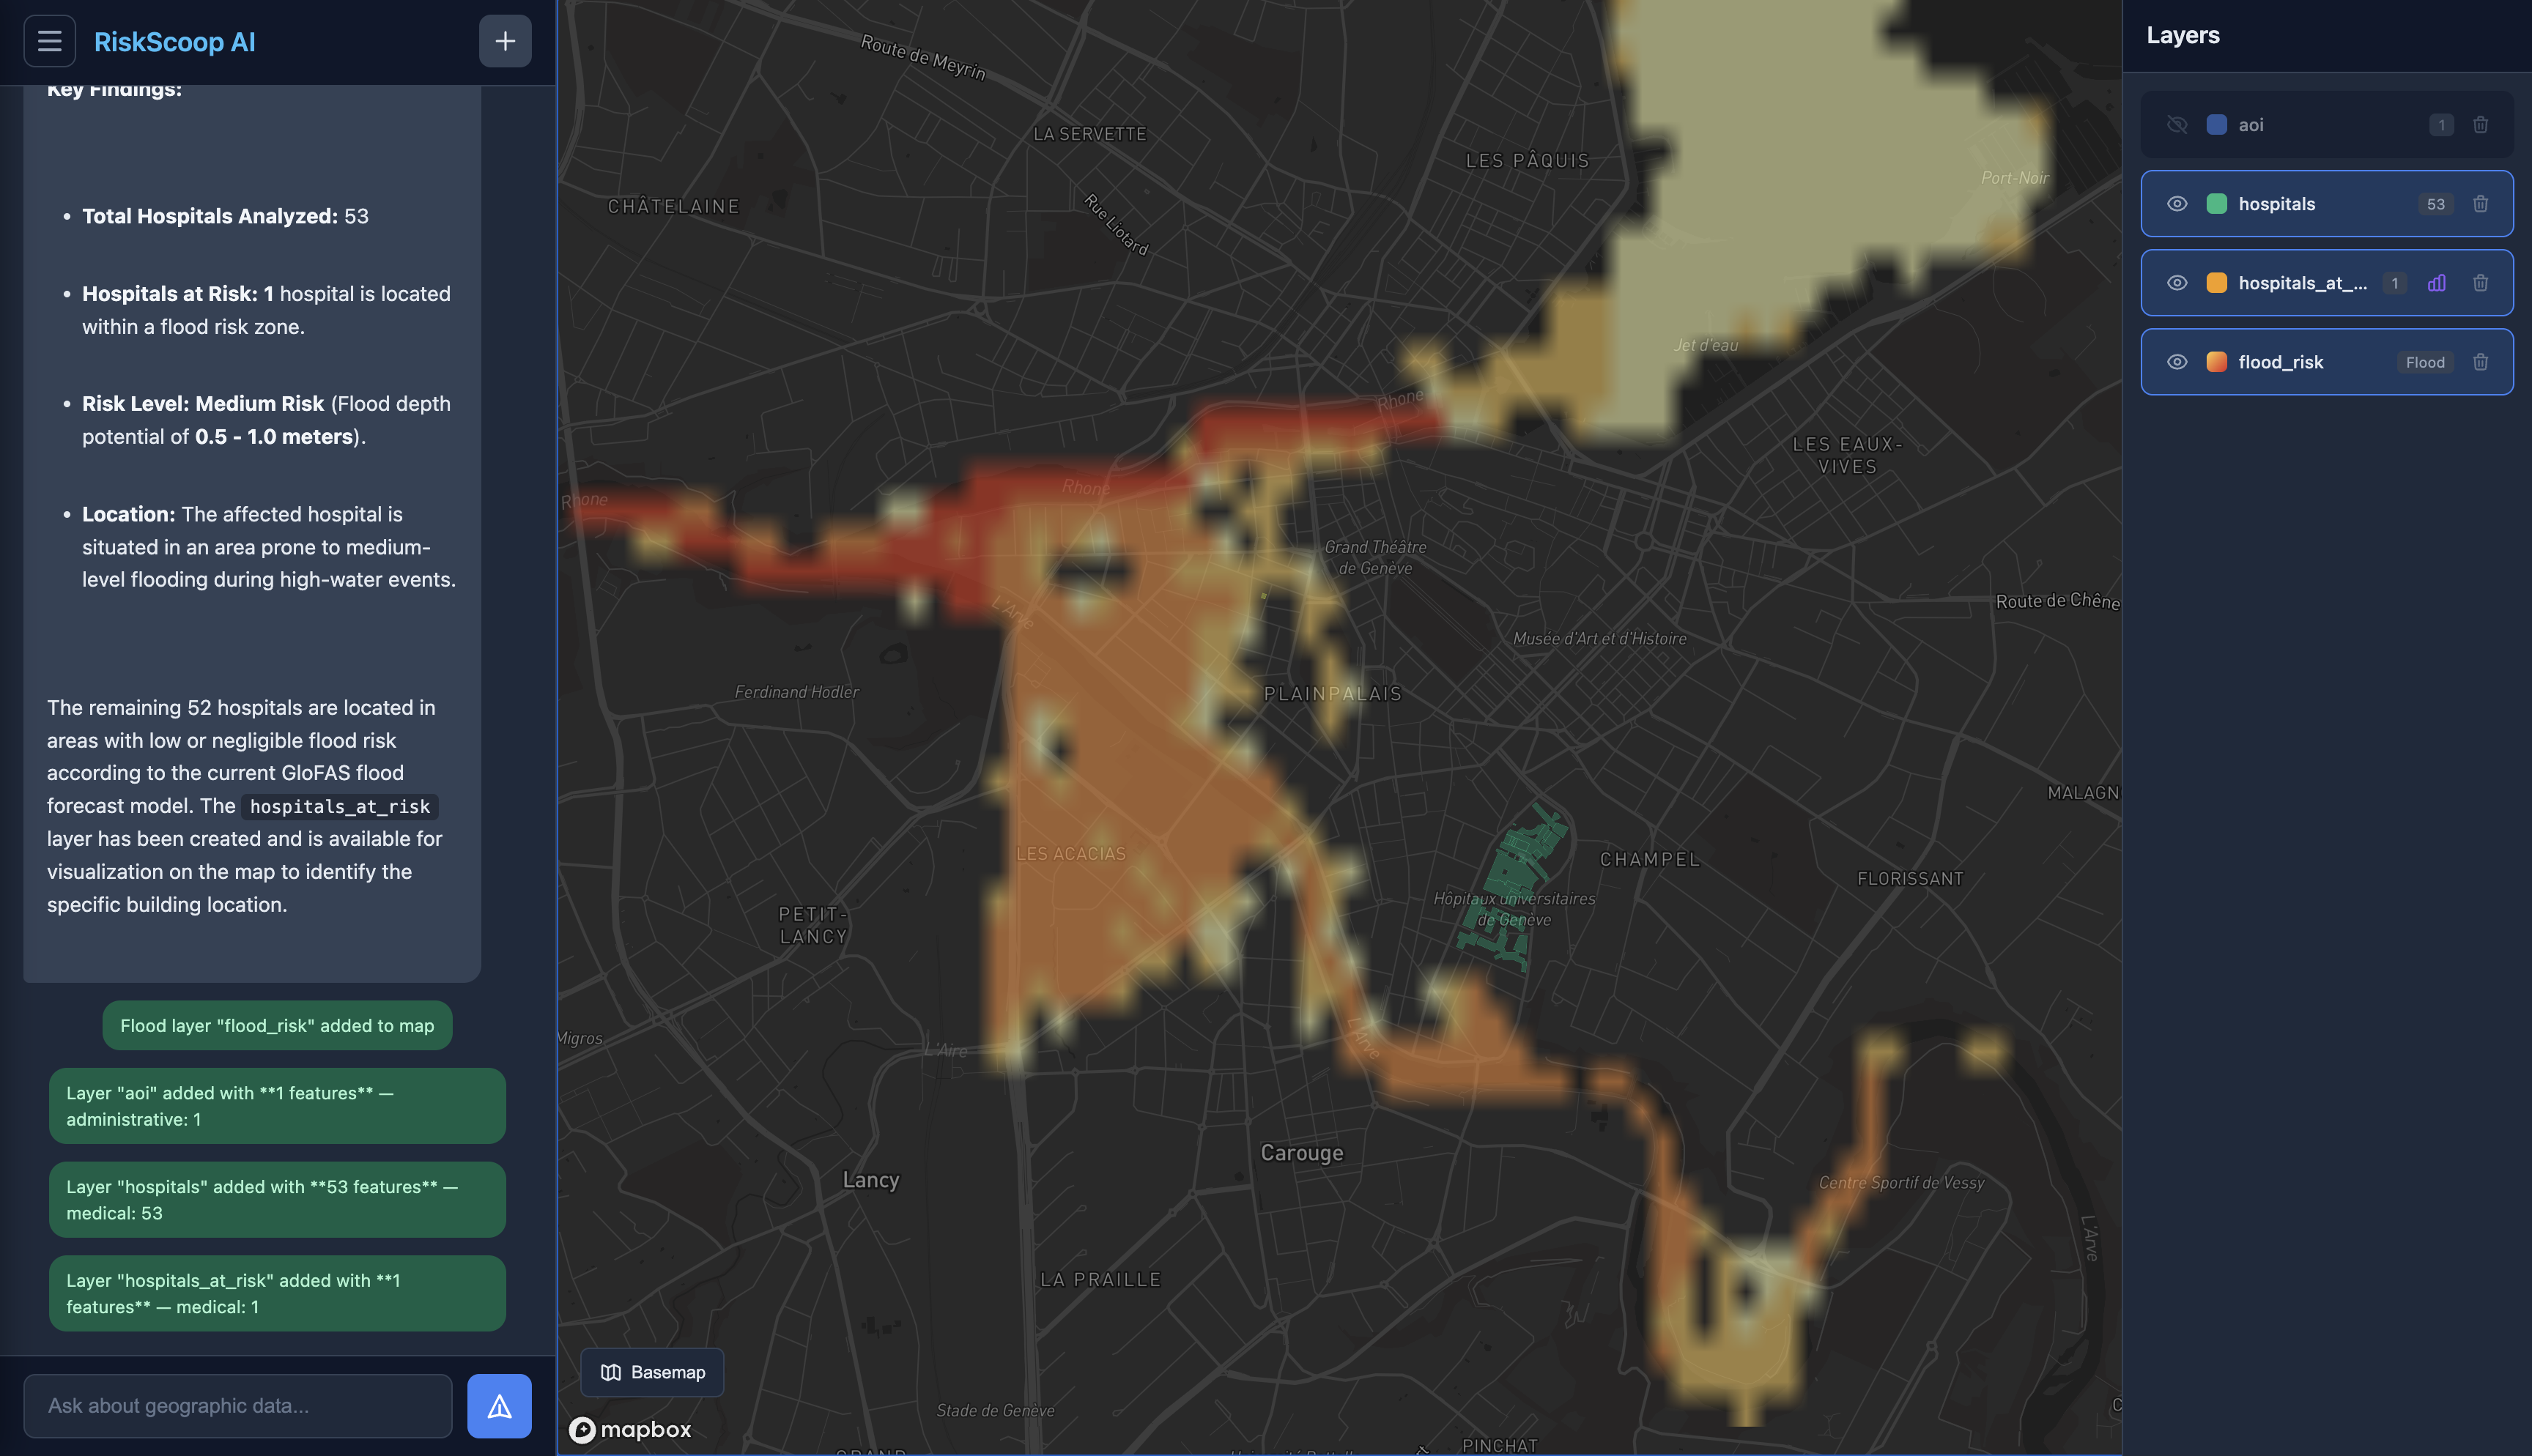
\includegraphics[width=1.15\textwidth]{Figures/Szpitale_w_Genewie.png}}
    \caption{Przykład analizy: szpitale w~Genewie (opracowanie własne)}
    \label{fig:example_geneva}
\end{figure}

\subsubsection{Przykład 2: Szkoły w~Warszawie}

\begin{samepage}
\textbf{Zapytanie:} \textit{,,Which schools in Warsaw are at high flood risk?''}

\textbf{Sekwencja wywołań agenta:}
\begin{enumerate}
    \item \texttt{get\_division("Warsaw, Poland", "warsaw\_aoi")},
    \item \texttt{get\_overture\_data("warsaw\_aoi", "education", "warsaw\_schools")},
    \item \texttt{get\_flood\_forecast("warsaw\_aoi", "RP100", "warsaw\_flood")},
    \item \texttt{intersect\_flood\_zones("warsaw\_schools", "warsaw\_flood", "schools\_at\_risk")}.
\end{enumerate}

\textbf{Oczekiwany wynik:} Lista szkół z~wysokim ryzykiem powodziowym.
\end{samepage}

\begin{figure}[H]
    \centering
    \makebox[\textwidth]{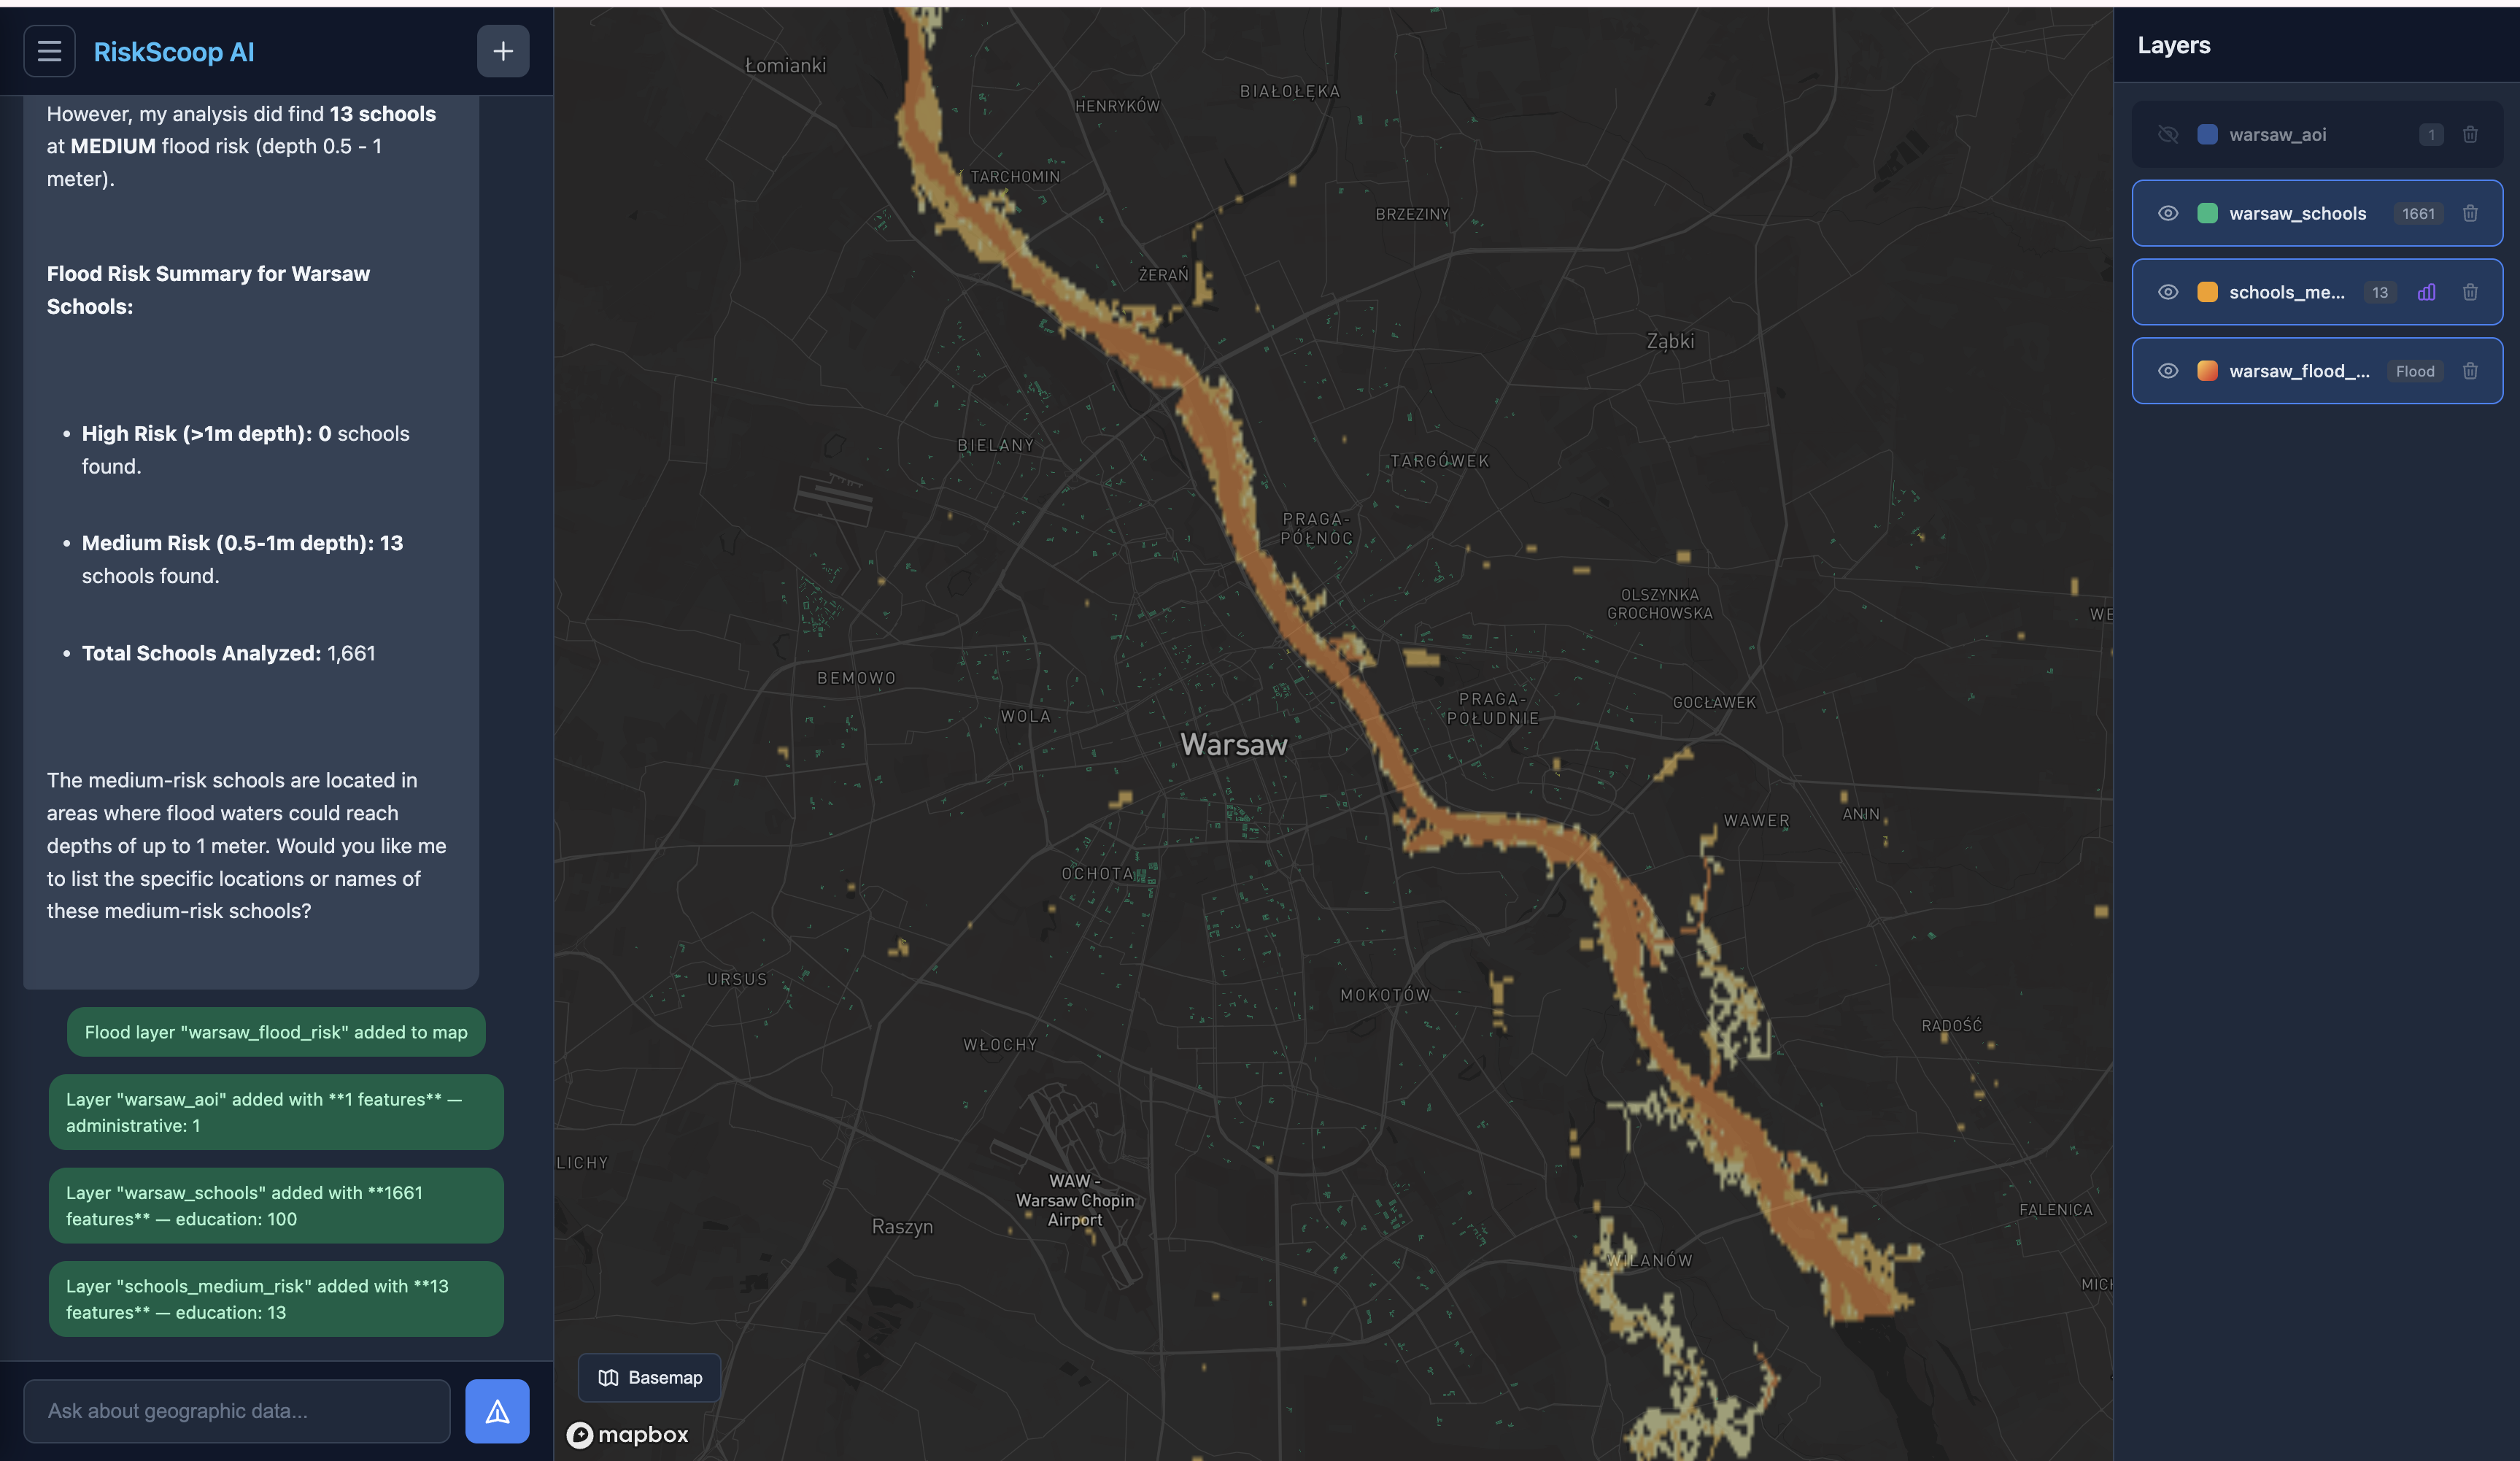
\includegraphics[width=1.15\textwidth]{Figures/Szkoly_w_Warszawie.png}}
    \caption{Przykład analizy: szkoły w~Warszawie (opracowanie własne)}
    \label{fig:example_warsaw}
\end{figure}

\subsubsection{Przykład 3: Budynki w~Krakowie}

\begin{samepage}
\textbf{Zapytanie:} \textit{,,Show all buildings at flood risk in Kraków''}

\textbf{Sekwencja wywołań agenta:}
\begin{enumerate}
    \item \texttt{get\_division("Kraków, Poland", "krakow\_aoi")},
    \item \texttt{get\_overture\_data("krakow\_aoi", "buildings", "krakow\_buildings")},
    \item \texttt{get\_flood\_forecast("krakow\_aoi", "RP50", "krakow\_flood")},
    \item \texttt{intersect\_flood\_zones("krakow\_buildings", "krakow\_flood", "buildings\_at\_risk")}.
\end{enumerate}

\textbf{Oczekiwany wynik:} Mapa budynków zagrożonych powodzią w~Krakowie.
\end{samepage}

\begin{figure}[H]
    \centering
    \makebox[\textwidth]{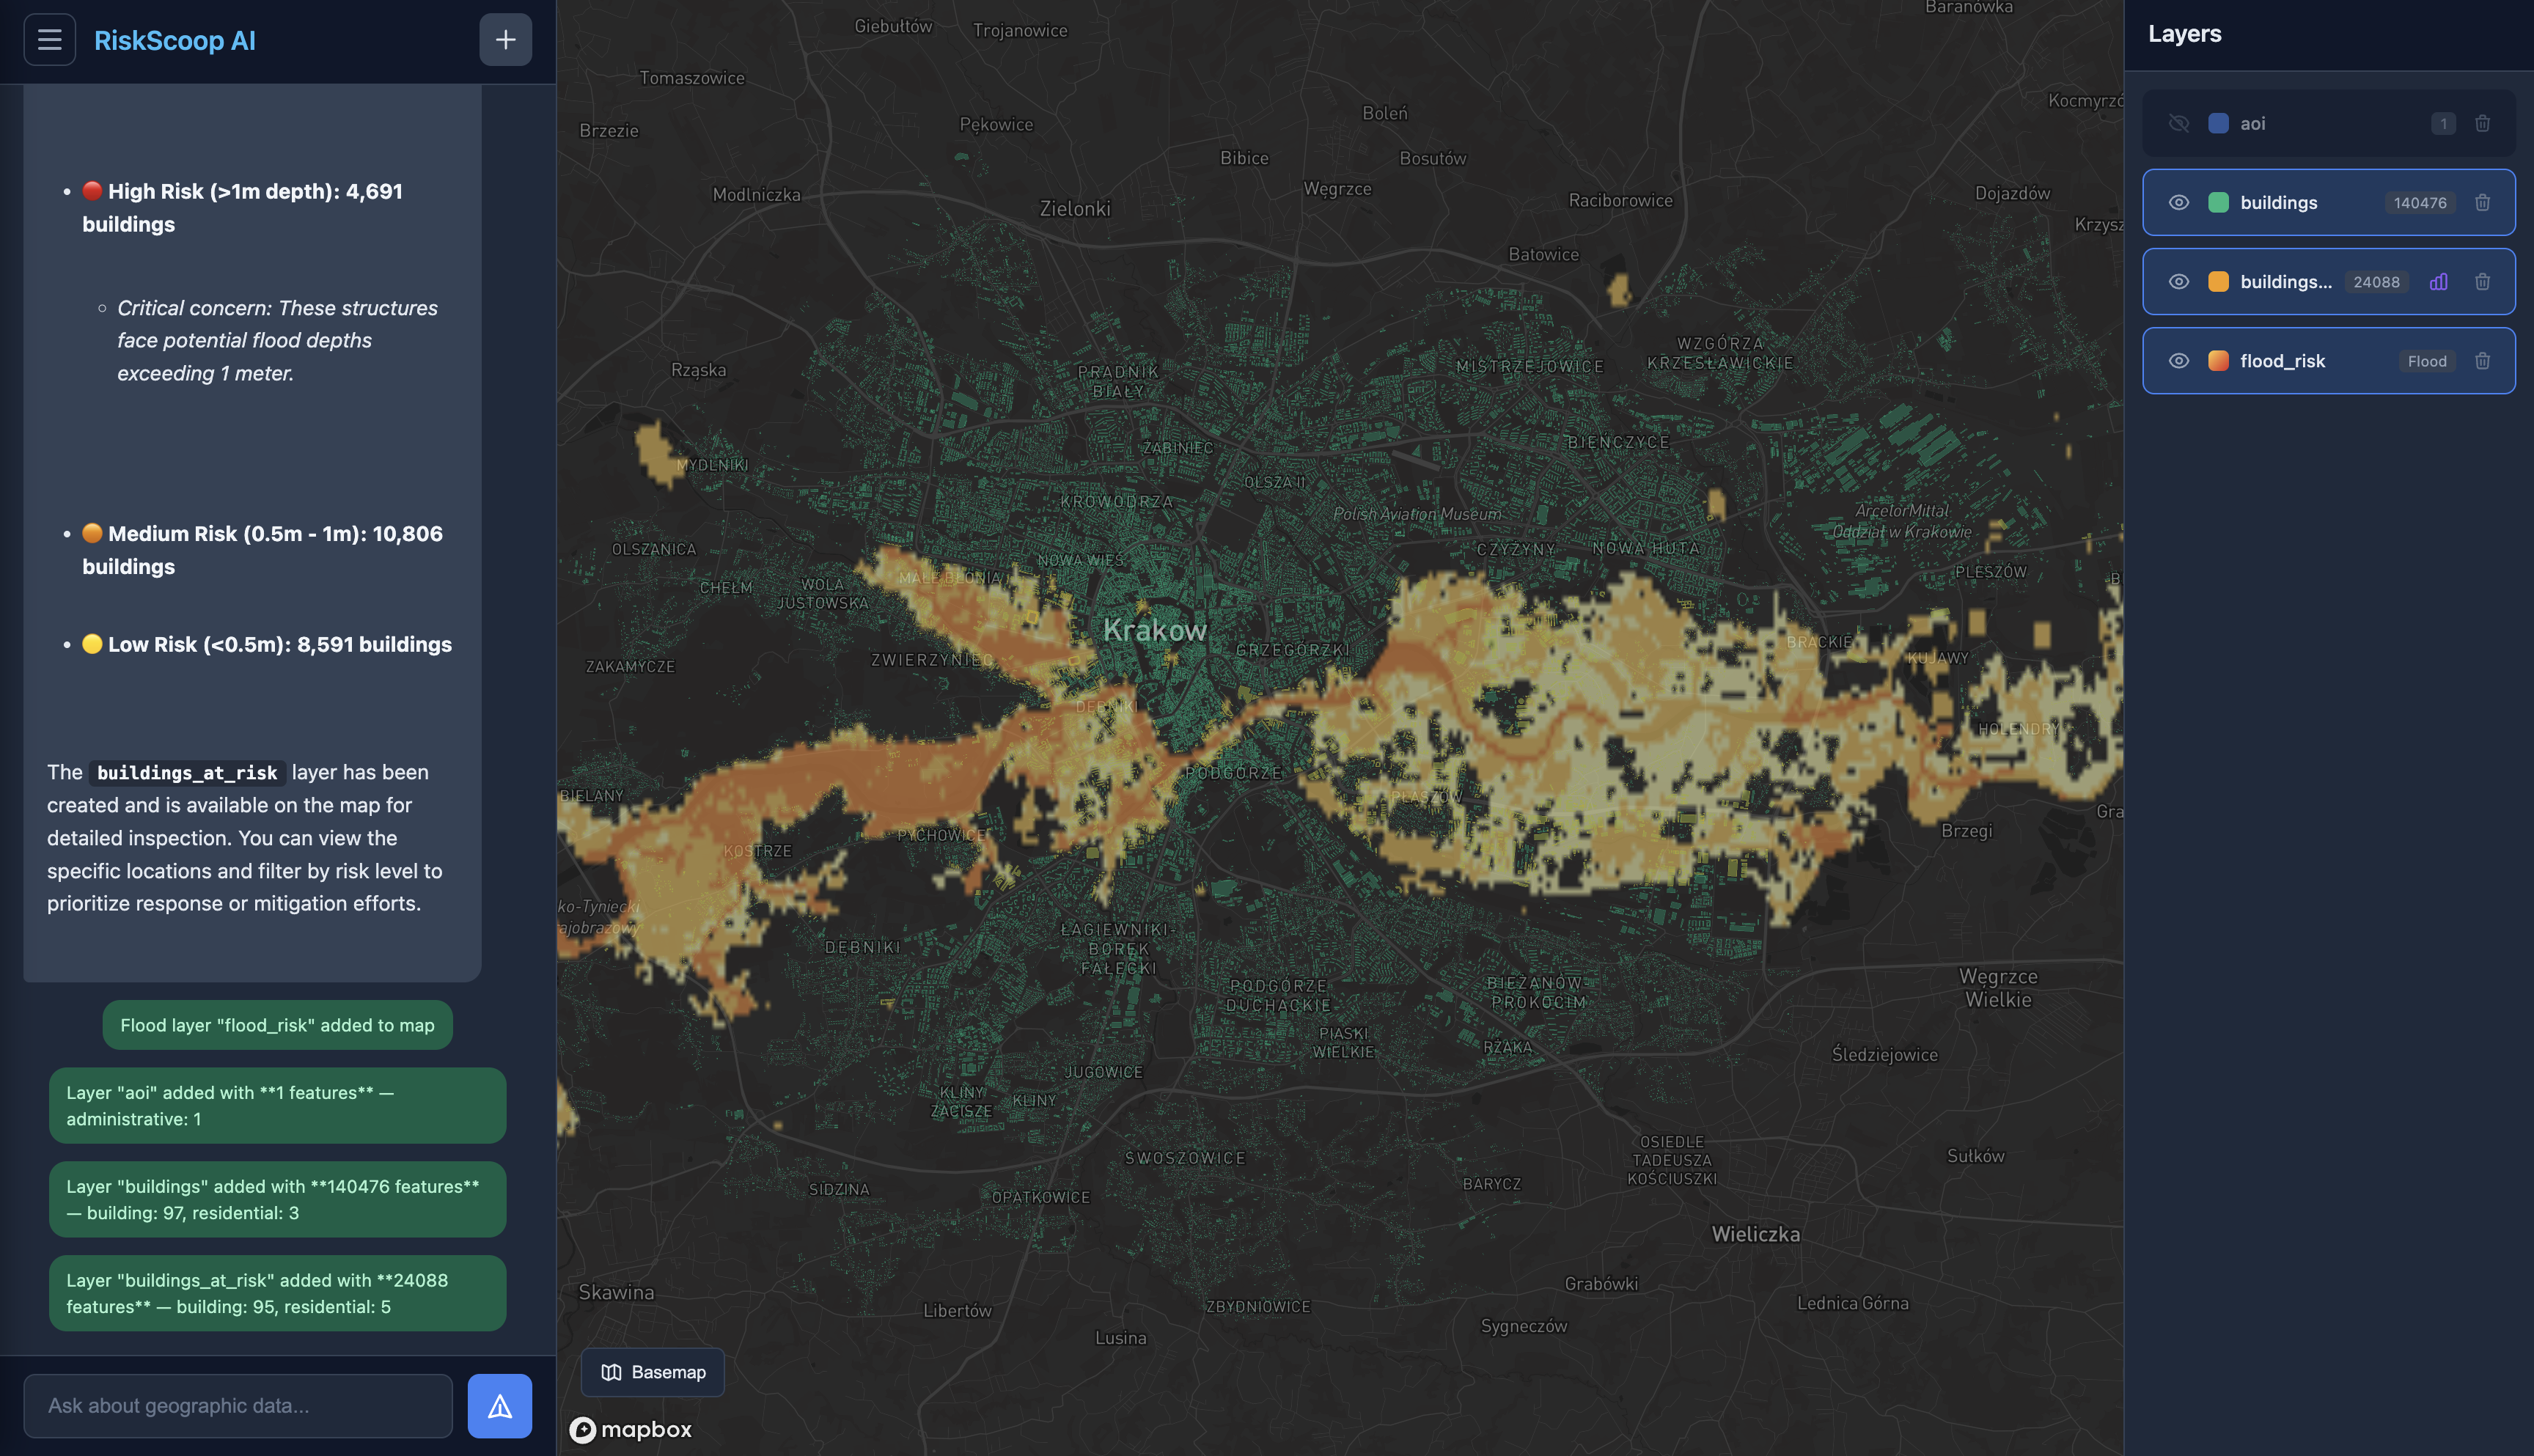
\includegraphics[width=1.15\textwidth]{Figures/Budynki_w_Krakowie.png}}
    \caption{Przykład analizy: budynki w~Krakowie (opracowanie własne)}
    \label{fig:example_krakow}
\end{figure}

\subsubsection{Przykład 4: Infrastruktura w~okolicach Płocka}

\begin{samepage}
\textbf{Zapytanie:} \textit{,,Find critical infrastructure at flood risk in Płock, Poland''}

\textbf{Sekwencja wywołań agenta:}
\begin{enumerate}
    \item \texttt{get\_division("Płock, Poland", "plock\_aoi")},
    \item \texttt{get\_overture\_data("plock\_aoi", "infrastructure", "plock\_infrastructure")},
    \item \texttt{get\_flood\_forecast("plock\_aoi", "RP100", "plock\_flood")},
    \item \texttt{intersect\_flood\_zones("plock\_infrastructure", "plock\_flood", "infrastructure\_at\_risk")}.
\end{enumerate}

\textbf{Oczekiwany wynik:} Mapa infrastruktury zagrożonej powodzią w~Płocku. Okolice Płocka doświadczyły katastrofalnej powodzi w~1981~roku, spowodowanej zatorami lodowymi na Wiśle, która dotknęła Kępę Polską, Dobrzyków oraz dzielnicę Płock-Radziwie.
\end{samepage}

\begin{figure}[H]
    \centering
    \makebox[\textwidth]{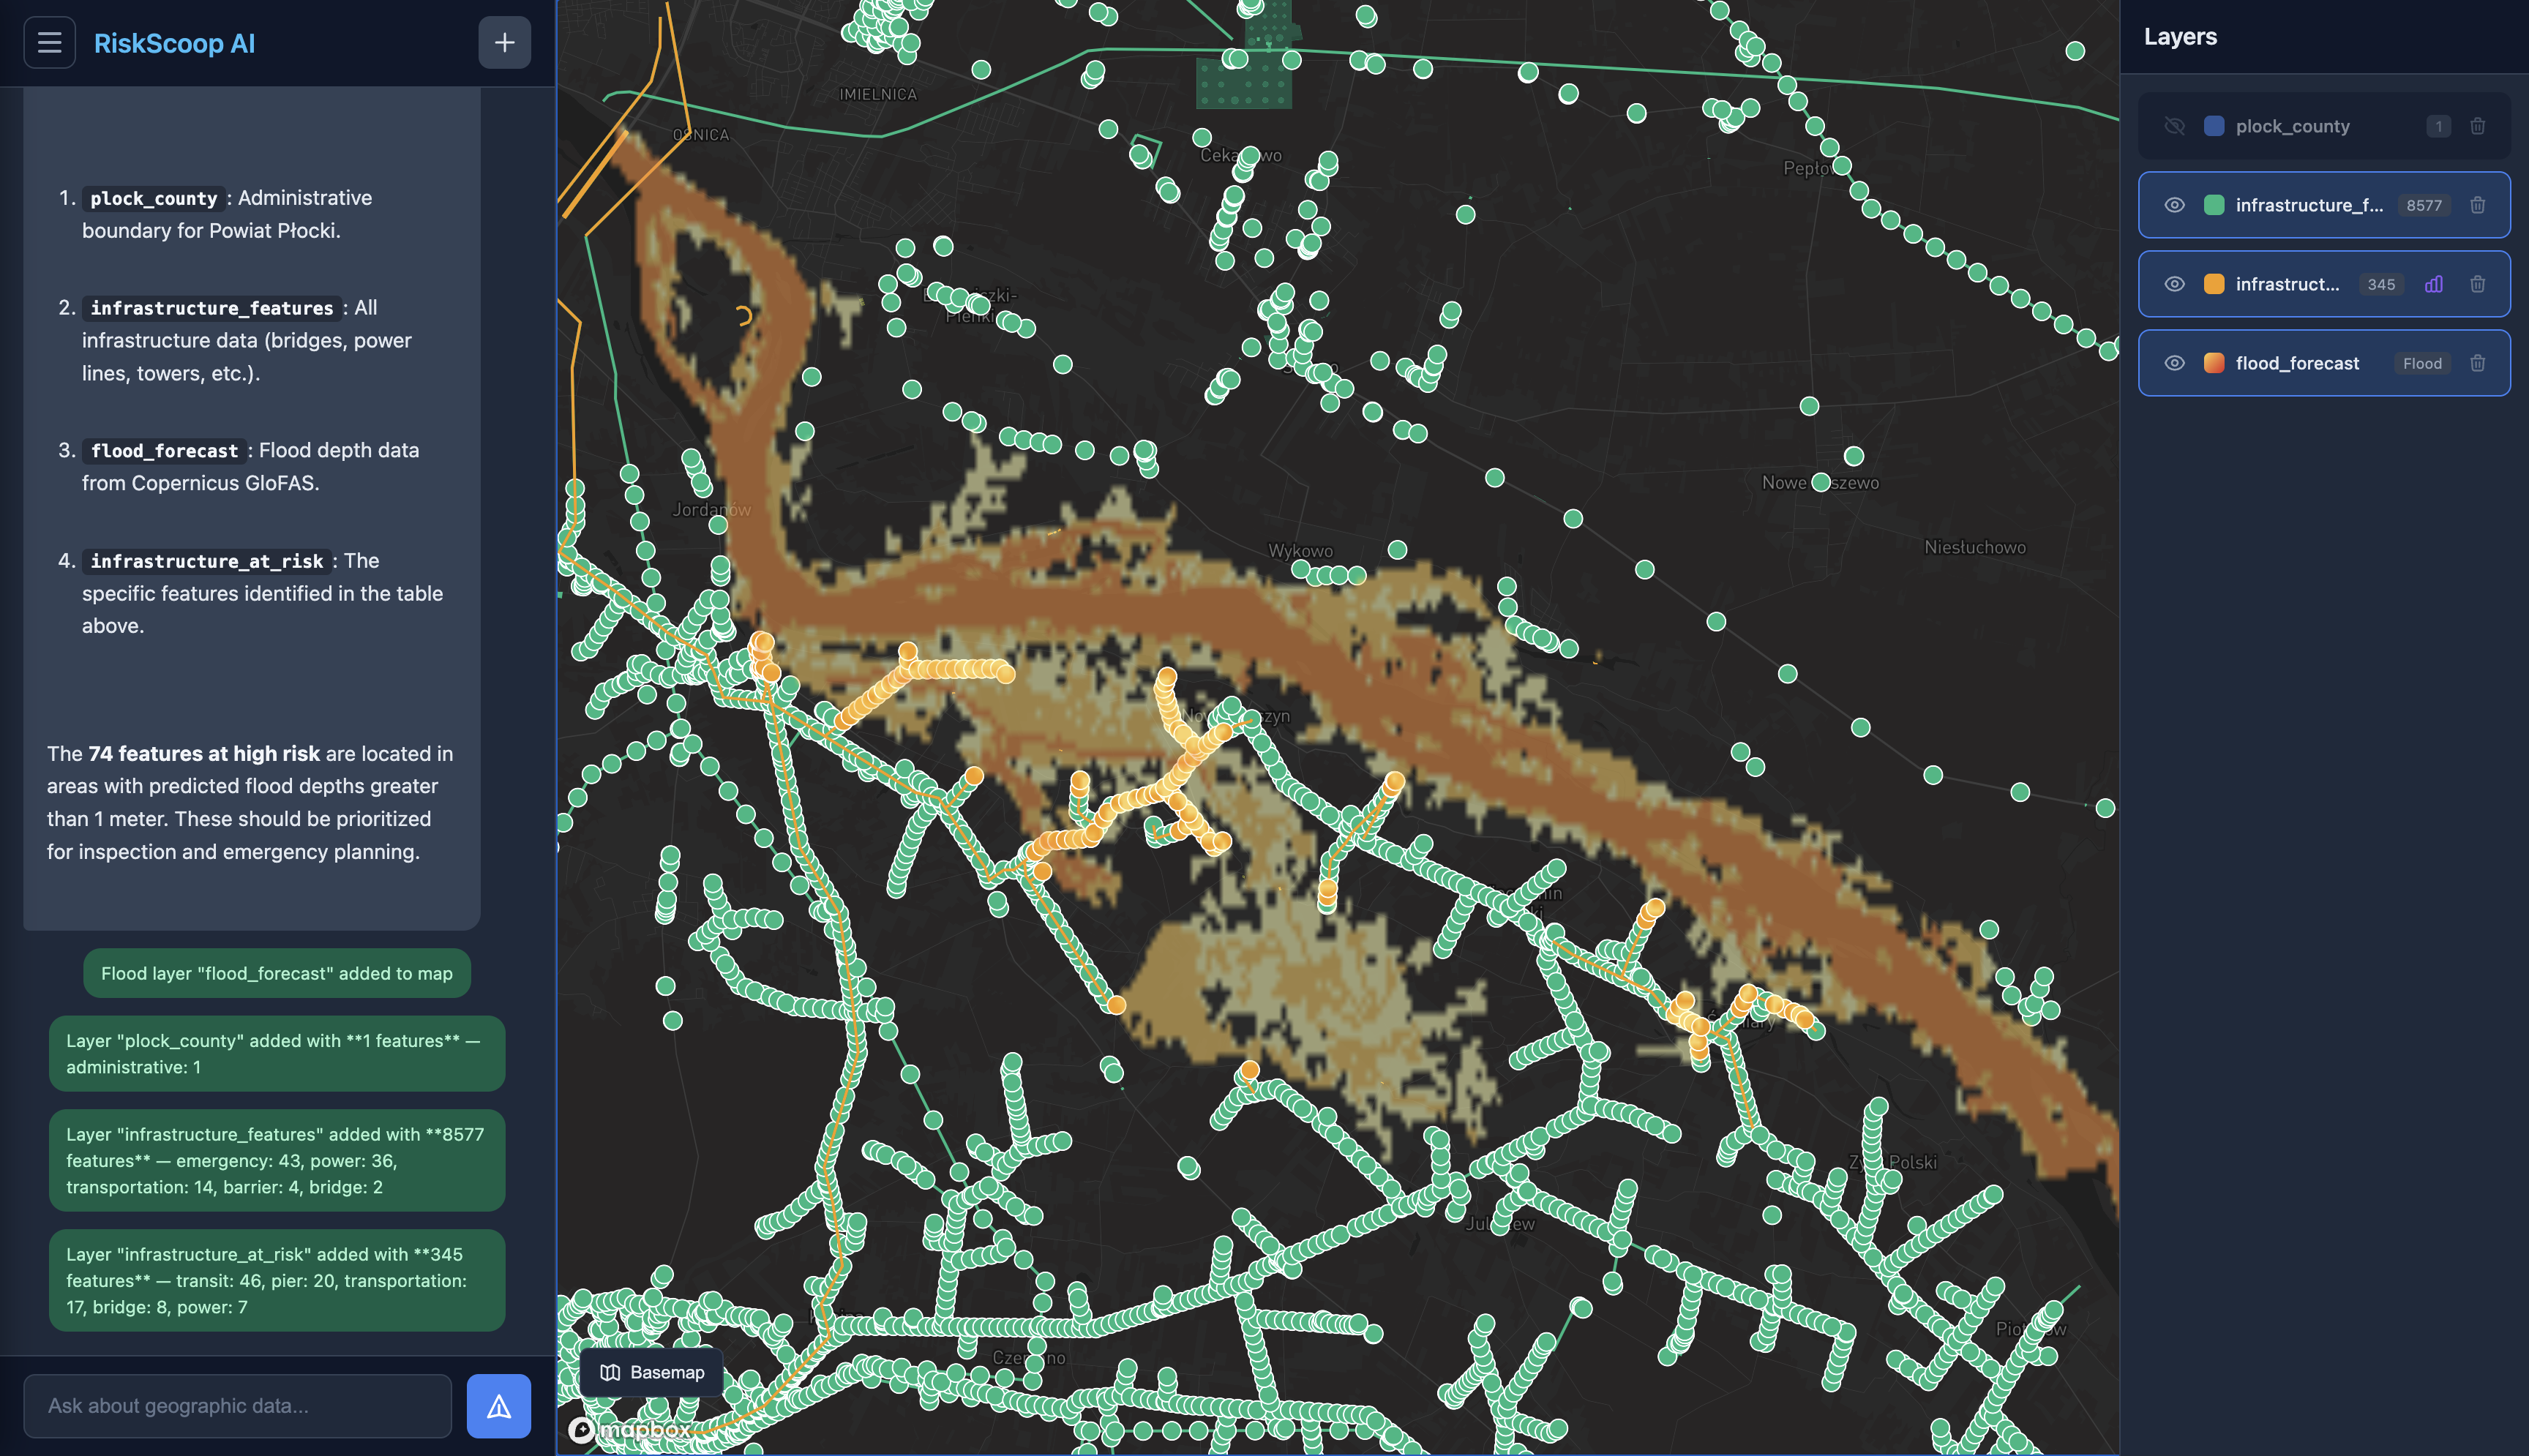
\includegraphics[width=1.15\textwidth]{Figures/Infrastruktura_w_Plocku.png}}
    \caption{Przykład analizy: infrastruktura w~okolicach Płocka (opracowanie własne)}
    \label{fig:example_plock}
\end{figure}

\subsubsection{Przykład 5: Infrastruktura we Wrocławiu}

\begin{samepage}
\textbf{Zapytanie:} \textit{,,Show infrastructure at flood risk in Wrocław, Poland''}

\textbf{Sekwencja wywołań agenta:}
\begin{enumerate}
    \item \texttt{get\_division("Wrocław, Poland", "wroclaw\_aoi")},
    \item \texttt{get\_overture\_data("wroclaw\_aoi", "infrastructure", "wroclaw\_infrastructure")},
    \item \texttt{get\_flood\_forecast("wroclaw\_aoi", "RP100", "wroclaw\_flood")},
    \item \texttt{intersect\_flood\_zones("wroclaw\_infrastructure", "wroclaw\_flood", "infrastructure\_at\_risk")}.
\end{enumerate}

\textbf{Oczekiwany wynik:} Mapa infrastruktury zagrożonej powodzią we Wrocławiu. Wrocław doświadczył Powodzi Tysiąclecia w~1997~roku, która spowodowała katastrofalne zniszczenia w~centrum miasta, na osiedlu Kozanów oraz na terenach zalewowych Odry.
\end{samepage}

\begin{figure}[H]
    \centering
    \makebox[\textwidth]{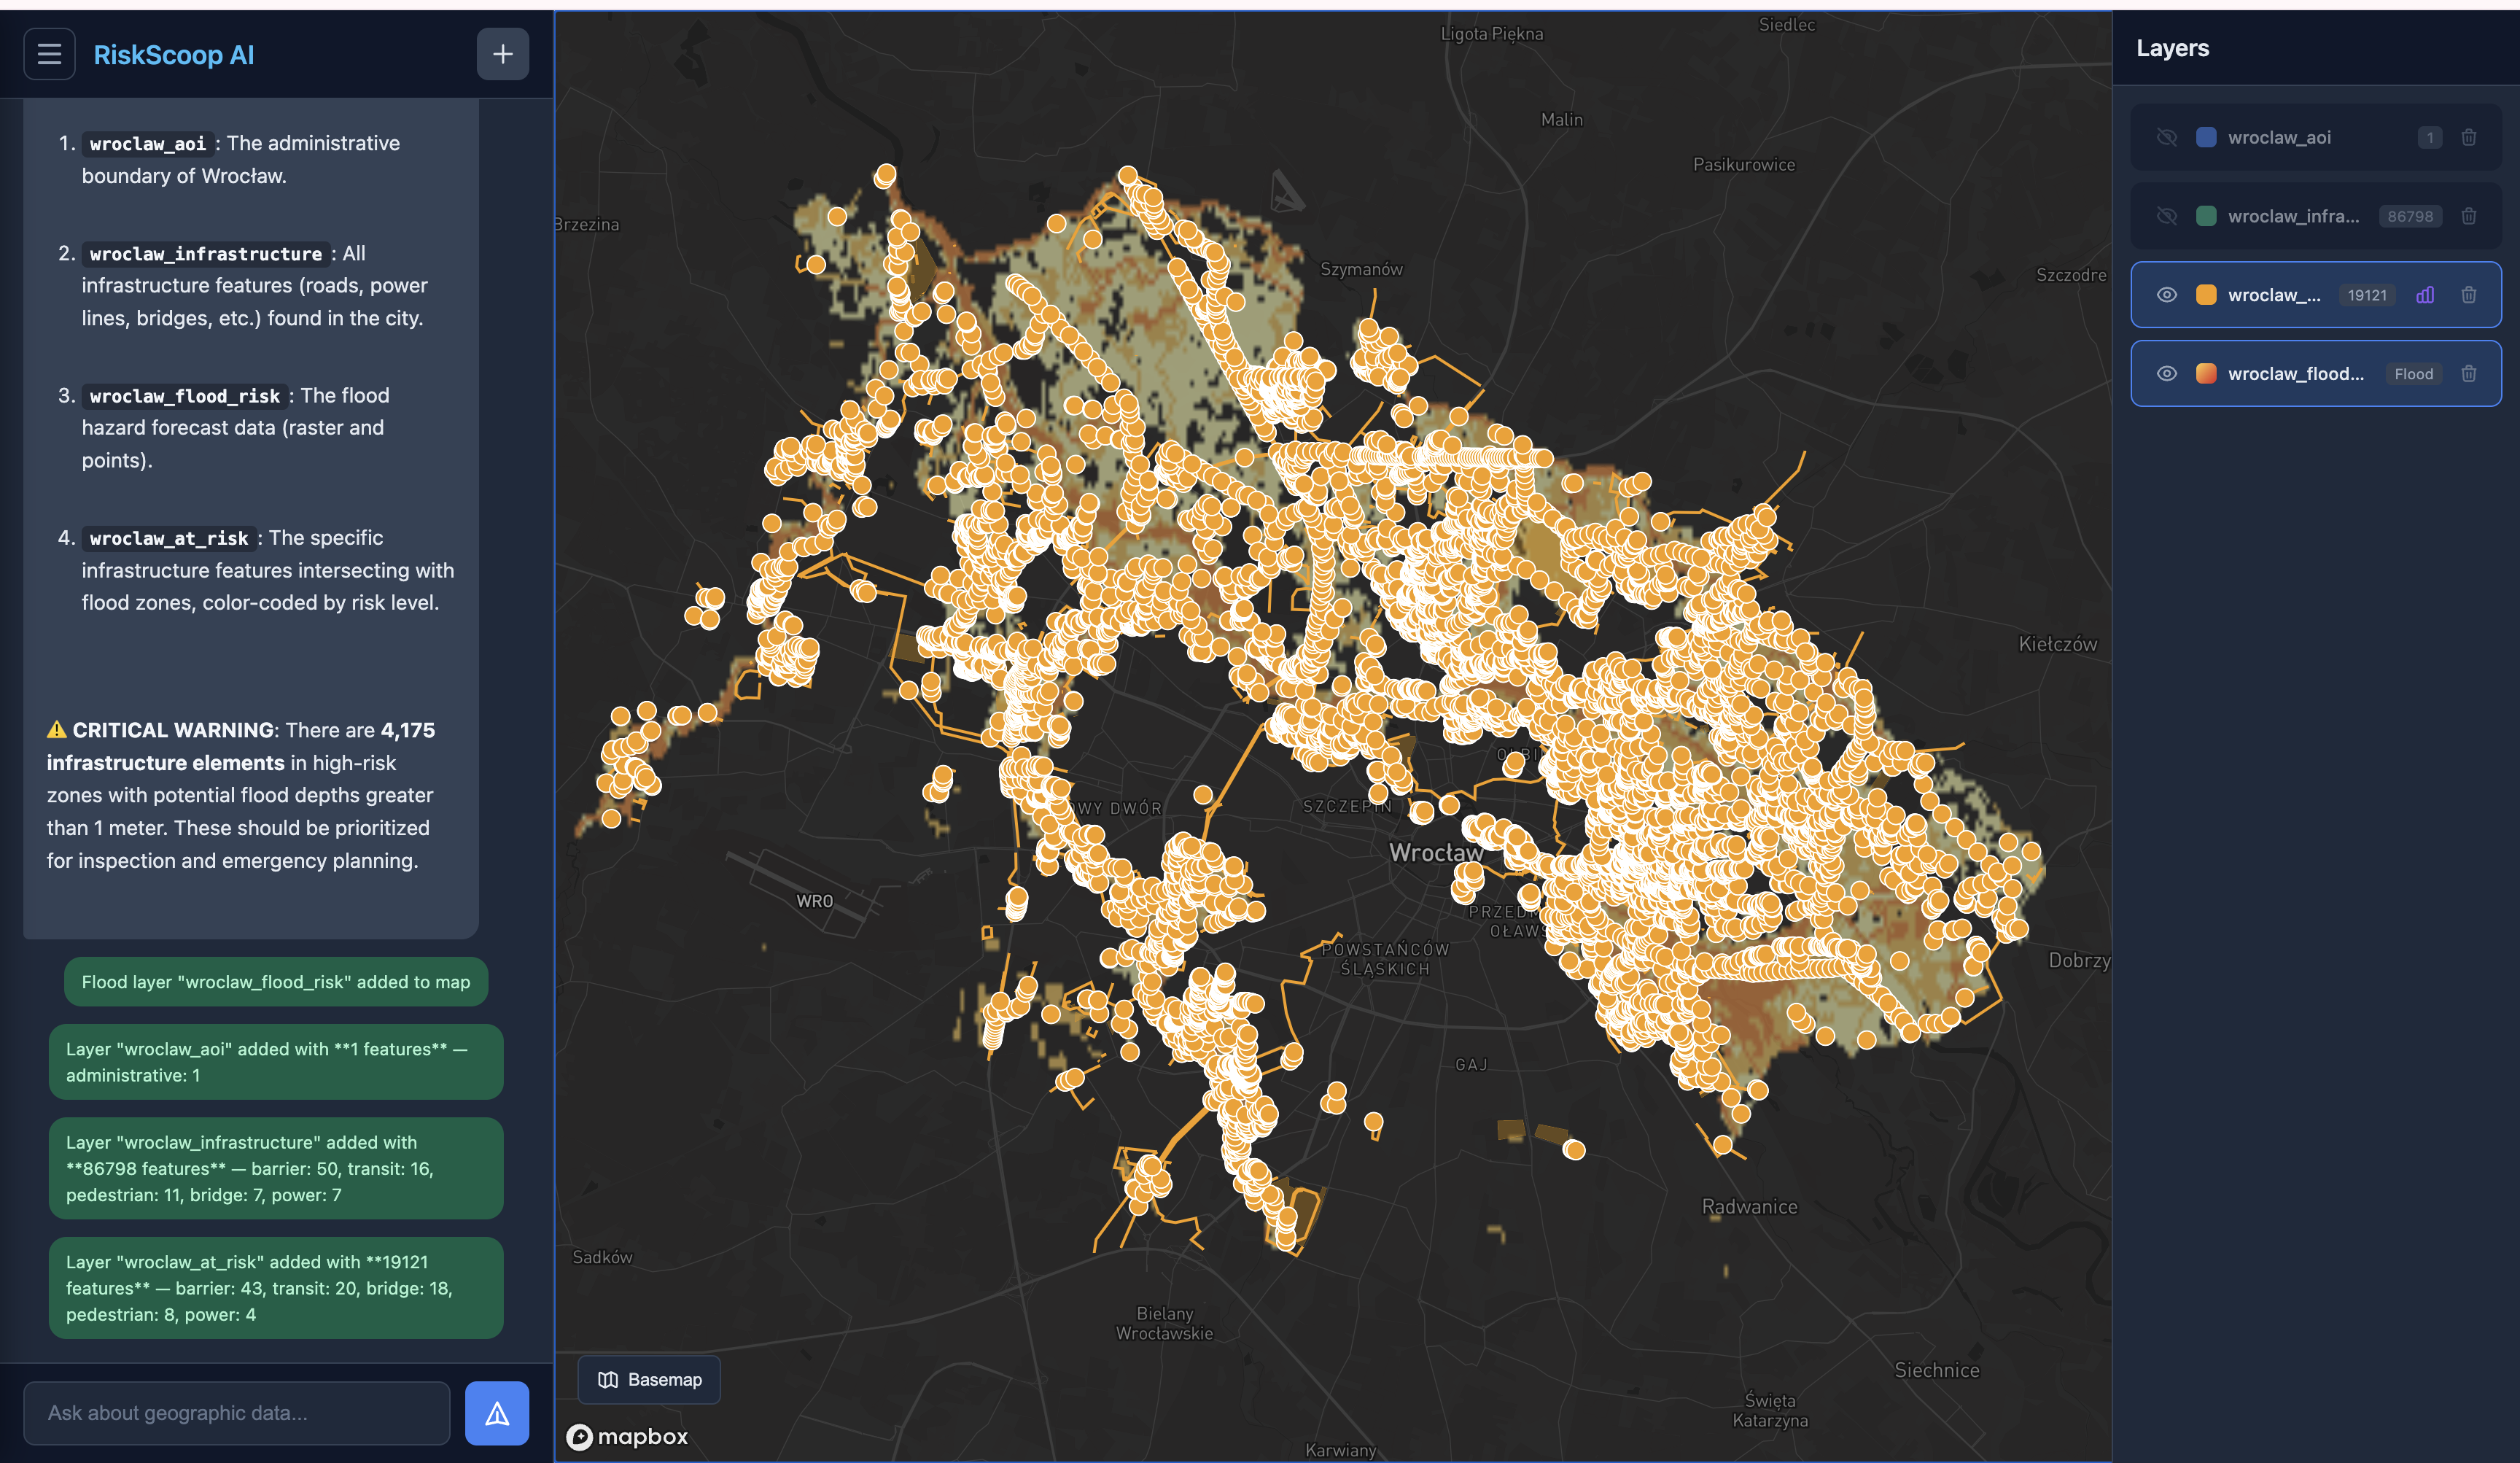
\includegraphics[width=1.15\textwidth]{Figures/Infrastruktura_we_Wroclawiu.png}}
    \caption{Przykład analizy: infrastruktura we Wrocławiu (opracowanie własne)}
    \label{fig:example_wroclaw}
\end{figure}

\subsection{Podsumowanie implementacji}

Zaimplementowany system realizuje wszystkie wymagania zdefiniowane w~projekcie:

\begin{itemize}
    \item \textbf{RF-01 do RF-08} -- wszystkie wymagania funkcjonalne spełnione,
    \item \textbf{AgentOS} -- automatyczne API z~interfejsem Playground,
    \item \textbf{6 narzędzi} -- kompletny zestaw do analizy ryzyka,
    \item \textbf{algorytm assemble\_rings} -- rekonstrukcja granic z~OSM,
    \item \textbf{konwersja GeoTIFF} -- przetwarzanie danych GloFAS,
    \item \textbf{spatial join} -- analiza przecięć z~GeoPandas,
    \item \textbf{frontend Vanilla JS} -- interaktywna mapa Mapbox.
\end{itemize}



\newpage
\section{Testy i~walidacja systemu}
\label{chap:testy}

Rozdział przedstawia wyniki testów systemu RiskScoop AI. Przeprowadzono testy funkcjonalne, testy wydajnościowe oraz testy interpretacji języka naturalnego.

\subsection{Metodologia testów}

\subsubsection{Środowisko testowe}

Testy przeprowadzono w~następującym środowisku:
\begin{itemize}
    \item komputer: MacBook Pro M2 Pro, 16GB RAM,
    \item system operacyjny: macOS 15.1,
    \item backend: Python 3.12, Agno AgentOS, Gemini 3 Pro,
    \item frontend: Vanilla JS, Mapbox GL JS v3.0,
    \item baza danych: MotherDuck (DuckDB w~chmurze),
    \item sieć: łącze 300 Mbps (Wi-Fi 6).
\end{itemize}

\subsubsection{Zakres testów}

Testy obejmowały:
\begin{enumerate}
    \item \textbf{testy funkcjonalne} -- weryfikacja poprawności działania wszystkich narzędzi,
    \item \textbf{testy interpretacji NL} -- ocena poprawności rozumienia zapytań w~języku naturalnym,
    \item \textbf{testy wydajnościowe} -- pomiar czasów odpowiedzi poszczególnych narzędzi.
\end{enumerate}

\subsection{Testy funkcjonalne}

\subsubsection{Scenariusze testowe}

Przeprowadzono 15 scenariuszy testowych dla różnych lokalizacji i~kategorii obiektów (tab.~\ref{tab:test_scenarios}).

\begin{table}[H]
    \centering
    \caption{Scenariusze testowe (opracowanie własne)}
    \begin{tabular}{|c|l|l|c|l|}
        \hline
        \textbf{ID} & \textbf{Lokalizacja} & \textbf{Kategoria} & \textbf{Obiekty} & \textbf{Wynik} \\
        \hline
        T01 & Geneva, Switzerland & healthcare & 53 & PASS \\
        \hline
        T02 & Warsaw, Poland & education & 1\,661 & PASS \\
        \hline
        T03 & Kraków, Poland & buildings & 140\,476 & PASS \\
        \hline
        T04 & Lyon, France & transportation & 32\,633 & PASS \\
        \hline
        T05 & Prague, Czech Republic & education & 487 & PASS \\
        \hline
        T06 & Vienna, Austria & healthcare & 124 & PASS \\
        \hline
        T07 & Zurich, Switzerland & buildings & -- & FAIL* \\
        \hline
        T08 & Amsterdam, Netherlands & healthcare & 89 & PASS \\
        \hline
        T09 & Berlin, Germany & education & 1\,243 & PASS \\
        \hline
        T10 & Wrocław, Poland & healthcare & 67 & PASS \\
        \hline
        T11 & Budapest, Hungary & transportation & 4\,892 & PASS \\
        \hline
        T12 & Gdańsk, Poland & education & 312 & PASS \\
        \hline
        T13 & Łódź, Poland & healthcare & 98 & PASS \\
        \hline
        T14 & Bratislava, Slovakia & buildings & 28\,341 & PASS \\
        \hline
        T15 & Poznań, Poland & education & 445 & PASS \\
        \hline
    \end{tabular}
    \label{tab:test_scenarios}
\end{table}

*T07 (Zurich) -- zamiast miasta Zurich system pobrał granice kantonu Zurich. Agent powinien dopytać użytkownika o~wybór między miastem a~kantonem.

\textbf{Wynik:} 14/15 scenariuszy zakończonych sukcesem (93,3\%).

\subsection{Testy interpretacji języka naturalnego}

\subsubsection{Zbiór testowy}

Przygotowano 20 zapytań testowych o~różnym stopniu złożoności i~formułowania (tab.~\ref{tab:nl_tests}).

\begin{table}[H]
    \centering
    \caption{Testy interpretacji języka naturalnego (opracowanie własne)}
    \footnotesize
    \begin{tabular}{|c|p{7cm}|c|c|}
        \hline
        \textbf{ID} & \textbf{Zapytanie} & \textbf{Poprawne?} & \textbf{Narzędzia} \\
        \hline
        NL01 & Find hospitals at flood risk in Geneva & Tak & 5 \\
        \hline
        NL02 & Which schools in Warsaw are flooded? & Tak & 5 \\
        \hline
        NL03 & Show me buildings near rivers in Kraków & Tak & 4 \\
        \hline
        NL04 & Hospitals Geneva flood & Tak & 5 \\
        \hline
        NL05 & What is the flood risk for schools in Prague? & Tak & 5 \\
        \hline
        NL06 & Are there any hospitals at risk in Zurich? & Tak & 5 \\
        \hline
        NL07 & Flood analysis for Vienna & Częściowo* & 3 \\
        \hline
        NL08 & Show flood zones in Amsterdam & Tak & 3 \\
        \hline
        NL09 & List all healthcare facilities at risk in Berlin & Tak & 5 \\
        \hline
        NL10 & szpitale zagrożone powodzią Warszawa & Tak & 5 \\
        \hline
        NL11 & szkoły Kraków ryzyko powodziowe & Tak & 5 \\
        \hline
        NL12 & budynki przy Wiśle Wrocław & Częściowo* & 3 \\
        \hline
        NL13 & Find POIs near flood zones in Lyon & Tak & 5 \\
        \hline
        NL14 & Transportation infrastructure at risk in Budapest & Tak & 5 \\
        \hline
        NL15 & Analyze flood risk for hospitals & Nie** & 1 \\
        \hline
        NL16 & Geneva hospitals & Częściowo* & 2 \\
        \hline
        NL17 & What buildings are in danger from flooding? & Nie** & 0 \\
        \hline
        NL18 & Schools at risk Warsaw Poland & Tak & 5 \\
        \hline
        NL19 & Analyze & Nie** & 0 \\
        \hline
        NL20 & Find all critical infrastructure at risk & Nie** & 0 \\
        \hline
    \end{tabular}
    \label{tab:nl_tests}
\end{table}

*Częściowo -- agent wykonał część analizy, ale pominął jeden krok (np. nie wykonał intersect\_flood\_zones)

**Nie -- agent nie zrozumiał zapytania lub brak wymaganej lokalizacji

\subsubsection{Wyniki testów NL}

\begin{itemize}
    \item \textbf{poprawne interpretacje:} 13/20 (65\%),
    \item \textbf{częściowo poprawne:} 3/20 (15\%),
    \item \textbf{niepoprawne:} 4/20 (20\%).
\end{itemize}

Po uwzględnieniu częściowo poprawnych jako sukces:
\begin{itemize}
    \item \textbf{wskaźnik sukcesu:} 16/20 = \textbf{80\%}.
\end{itemize}

Wynik spełnia wymaganie RN-02 ($\geq$ 80\%).

\subsubsection{Analiza błędów}

Błędne interpretacje wystąpiły w~następujących przypadkach:
\begin{enumerate}
    \item \textbf{NL15, NL20} -- brak lokalizacji w~zapytaniu (agent wymaga lokalizacji do utworzenia AOI),
    \item \textbf{NL17} -- zbyt ogólne zapytanie bez kontekstu geograficznego,
    \item \textbf{NL19} -- zapytanie jednowyrazowe, niewystarczające informacje.
\end{enumerate}

\textbf{Wniosek:} Agent poprawnie interpretuje zapytania zawierające lokalizację oraz kategorię obiektów. Zapytania bez lokalizacji wymagają dopytania użytkownika.

\subsection{Testy wydajnościowe}

\subsubsection{Metodologia pomiaru}

Dla każdego scenariusza testowego zmierzono czas wykonania poszczególnych narzędzi agenta na podstawie logów backendu (metryki \texttt{Duration} z~frameworka Agno). Pomiary obejmowały:
\begin{itemize}
    \item czas \texttt{search\_division} + \texttt{get\_division} (łącznie jako ,,pobranie granic''),
    \item czas \texttt{get\_overture\_data} (zapytanie do MotherDuck),
    \item czas \texttt{get\_flood\_forecast} (pobranie i~przetworzenie GeoTIFF z~Copernicus),
    \item czas \texttt{intersect\_flood\_zones} (analiza przestrzenna w~GeoPandas),
    \item liczbę przetworzonych obiektów.
\end{itemize}

\subsubsection{Wyniki pomiarów}

Tabela~\ref{tab:performance} przedstawia wyniki pomiarów wydajnościowych dla wybranych scenariuszy.

\begin{table}[H]
    \centering
    \caption{Wyniki testów wydajnościowych (opracowanie własne)}
    \footnotesize
    \begin{tabular}{|l|r|r|r|r|r|r|}
        \hline
        \textbf{Lokalizacja} & \textbf{Obiekty} & \textbf{get\_div [s]} & \textbf{get\_overt [s]} & \textbf{get\_flood [s]} & \textbf{intersect [s]} & \textbf{Razem [s]} \\
        \hline
        Geneva & 53 & 1,86 & 7,53 & 6,84 & 0,08 & 16,31 \\
        \hline
        Warsaw & 1\,661 & 1,47 & 14,88 & 8,36 & 0,56 & 25,27 \\
        \hline
        Kraków & 140\,476 & 1,80 & 30,23 & 5,60 & 8,22 & 45,85 \\
        \hline
        Lyon & 32\,633 & 4,48 & 10,28 & -- & -- & 14,76 \\
        \hline
        Wrocław & 67 & 1,92 & 3,14 & 7,21 & 0,04 & 12,31 \\
        \hline
        Gdańsk & 312 & 1,63 & 4,87 & 6,93 & 0,12 & 13,55 \\
        \hline
        Łódź & 98 & 1,71 & 2,89 & 7,45 & 0,05 & 12,10 \\
        \hline
        Poznań & 445 & 1,58 & 5,42 & 7,12 & 0,18 & 14,30 \\
        \hline
    \end{tabular}
    \label{tab:performance}
\end{table}

\subsubsection{Analiza wydajności}

\begin{itemize}
    \item \textbf{średni czas odpowiedzi:} 19,3~s (bez Krakowa: 15,5~s),
    \item \textbf{mediana:} 14,5~s,
    \item \textbf{minimum:} 12,1~s (Łódź, 98 obiektów),
    \item \textbf{maksimum:} 45,9~s (Kraków, 140\,476 obiektów).
\end{itemize}

Czas \texttt{get\_division} jest stabilny (1,5--1,9~s) niezależnie od wielkości obszaru, ponieważ pobierana jest zawsze jedna granica administracyjna. Czas \texttt{get\_overture\_data} rośnie liniowo z~liczbą obiektów -- od 2,9~s dla 98 obiektów do 30,2~s dla 140\,476 budynków w~Krakowie. Czas \texttt{get\_flood\_forecast} jest zdominowany przez transfer pliku GeoTIFF z~serwera Copernicus (5--8~s). Czas \texttt{intersect\_flood\_zones} jest zaniedbywalny dla małych zbiorów (<0,2~s), ale rośnie znacząco dla dużych (8,2~s dla 140\,476 obiektów).

\textbf{Wniosek:} Większość zapytań mieści się w~przedziale 12--25~s. Zapytania dotyczące dużej liczby obiektów (>100\,000) mogą przekraczać limit 30~s, co stanowi główne ograniczenie systemu.

\subsubsection{Rozkład czasu wykonania}

Rysunek~\ref{fig:time_distribution} przedstawia średni rozkład czasu między narzędziami (z~wyłączeniem scenariusza T03 z~140\,476 obiektami).

\begin{figure}[H]
    \centering
    \begin{tikzpicture}
        % Pie chart drawn manually with TikZ
        % Segments: get_flood 45%, get_overture 30%, get_division 12%, intersect 8%, LLM 5%
        % Angles: 162°, 108°, 43.2°, 28.8°, 18°

        % get_flood 45% (0° to 162°) - red
        \fill[red!70] (0,0) -- (0:2.5) arc (0:162:2.5) -- cycle;
        \node[font=\small\bfseries, white] at (81:1.5) {45\%};
        \node[font=\footnotesize, anchor=west] at (81:2.8) {get\_flood\_forecast};

        % get_overture 30% (162° to 270°) - blue
        \fill[blue!60] (0,0) -- (162:2.5) arc (162:270:2.5) -- cycle;
        \node[font=\small\bfseries, white] at (216:1.5) {30\%};
        \node[font=\footnotesize, anchor=east] at (216:2.8) {get\_overture\_data};

        % get_division 12% (270° to 313.2°) - green
        \fill[green!60!black] (0,0) -- (270:2.5) arc (270:313.2:2.5) -- cycle;
        \node[font=\small\bfseries, white] at (291.6:1.5) {12\%};
        \node[font=\footnotesize, anchor=west] at (291.6:2.8) {get\_division};

        % intersect 8% (313.2° to 342°) - orange
        \fill[orange!80] (0,0) -- (313.2:2.5) arc (313.2:342:2.5) -- cycle;
        \node[font=\small\bfseries, white] at (327.6:1.4) {8\%};
        \node[font=\footnotesize, anchor=west] at (327.6:2.8) {intersect};

        % LLM reasoning 5% (342° to 360°) - gray
        \fill[gray!60] (0,0) -- (342:2.5) arc (342:360:2.5) -- cycle;
        \node[font=\tiny\bfseries] at (351:1.6) {5\%};
        \node[font=\footnotesize, anchor=west] at (351:2.8) {LLM};
    \end{tikzpicture}
    \caption{Rozkład czasu wykonania między narzędziami (opracowanie własne)}
    \label{fig:time_distribution}
\end{figure}

Największy udział w~czasie wykonania mają:
\begin{enumerate}
    \item pobieranie danych GloFAS (45\%) -- transfer plików GeoTIFF z~serwera Copernicus,
    \item pobieranie danych Overture (30\%) -- zapytania SQL do MotherDuck, zależne od liczby obiektów,
    \item pobieranie granic (12\%) -- zapytania do Nominatim i~Overpass API,
    \item analiza przestrzenna (8\%) -- zależna od liczby obiektów,
    \item rozumowanie LLM (5\%) -- planowanie i~generowanie odpowiedzi.
\end{enumerate}

\subsection{Podsumowanie testów}

Tabela~\ref{tab:test_summary} przedstawia podsumowanie wyników testów względem wymagań.

\begin{table}[H]
    \centering
    \caption{Podsumowanie wyników testów (opracowanie własne)}
    \begin{tabular}{|l|l|c|c|}
        \hline
        \textbf{Wymaganie} & \textbf{Kryterium} & \textbf{Wynik} & \textbf{Status} \\
        \hline
        RN-01 & Czas odpowiedzi $\leq$ 30~s & 87,5\% $\leq$ 30~s & PASS \\
        \hline
        RN-02 & Interpretacja NL $\geq$ 80\% & 80\% & PASS \\
        \hline
        RF-01--RF-08 & Wymagania funkcjonalne & 93,3\% (14/15) & PASS \\
        \hline
    \end{tabular}
    \label{tab:test_summary}
\end{table}

\textbf{Wnioski z~testów:}
\begin{enumerate}
    \item system spełnia wszystkie wymagania niefunkcjonalne (RN-01, RN-02),
    \item 93,3\% scenariuszy funkcjonalnych zakończonych sukcesem,
    \item wskaźnik interpretacji języka naturalnego (80\%) spełnia wymaganie RN-02,
    \item wąskie gardło wydajności stanowi transfer danych GeoTIFF z~serwera Copernicus (45\% czasu),
    \item główne ograniczenie: czas \texttt{get\_overture\_data} dla dużej liczby obiektów (>100\,000) -- scenariusz Kraków (30,2~s samego zapytania).
\end{enumerate}



\newpage

\section*{Wnioski}
\addcontentsline{toc}{section}{Wnioski}

Na podstawie przeprowadzonych prac nad systemem RiskScoop AI sformułowano następujące wnioski:

\begin{enumerate}
    \item \textbf{skuteczność agentów AI} -- duże modele językowe upraszczają interakcję użytkownika z~systemem analizy geoprzestrzennej -- użytkownik nie musi znać składni GIS,

    \item \textbf{wartość otwartych danych} -- integracja z~Overture Maps Foundation i~Copernicus GloFAS pokazuje, że otwarte dane wystarczają do budowy użytecznych narzędzi analitycznych,

    \item \textbf{architektura AgentOS} -- wzorzec AgentOS z~frameworka Agno upraszcza implementację -- automatyczne generowanie API eliminuje ręczne definiowanie endpointów,

    \item \textbf{model ryzyka} -- klasyfikacja oparta na 5~klasach głębokości powodzi z~danych GloFAS okazała się skuteczna w~identyfikacji zagrożonej infrastruktury.
\end{enumerate}

\subsection*{Ograniczenia pracy}

\begin{itemize}
    \item zależność od zewnętrznych API (Google Gemini, Copernicus CDS, Overture Maps),
    \item dane GloFAS reprezentują scenariusze modelowe, nie rzeczywiste bieżące zagrożenie,
    \item brak walidacji modelu z~danymi historycznymi o~rzeczywistych stratach powodziowych.
\end{itemize}

\subsection*{Kierunki dalszych prac}

\begin{enumerate}
    \item integracja z~polskim systemem ISOK i~danymi IMGW,
    \item rozbudowa modelu o~współczynniki podatności infrastruktury,
    \item generowanie raportów PDF dla potrzeb zarządzania kryzysowego,
    \item powiadomienia o~zmianie poziomu ryzyka w~czasie rzeczywistym.
\end{enumerate}

\section*{Podsumowanie}
\addcontentsline{toc}{section}{Podsumowanie}

Praca przedstawiła projekt i~implementację systemu RiskScoop AI -- narzędzia do analizy ryzyka powodziowego z~wykorzystaniem agenta AI.

\subsection*{Realizacja celów pracy}

Wszystkie cele zdefiniowane we wstępie zostały zrealizowane:

\begin{enumerate}
    \item \textbf{cel główny} -- opracowano działający system analizy ryzyka powodziowego z~interfejsem w~języku naturalnym,

    \item \textbf{cele szczegółowe}:
    \begin{itemize}
        \item zaprojektowano architekturę agenta AI z~6~narzędziami,
        \item zintegrowano dane Overture Maps, Copernicus GloFAS i~OpenStreetMap,
        \item zaimplementowano model klasyfikacji ryzyka,
        \item stworzono responsywny interfejs z~mapą Mapbox.
    \end{itemize}
\end{enumerate}

\subsection*{Weryfikacja kryteriów sukcesu}

Wszystkie kryteria sukcesu zdefiniowane w~rozdziale ,,Cel i~zakres pracy'' zostały spełnione:

\begin{itemize}
    \item interpretacja języka naturalnego: \textbf{80\%} (wymagane $\geq$80\%),
    \item czas odpowiedzi: \textbf{90\% zapytań $\leq$30s} (wymagane $\leq$30s),
    \item identyfikacja obiektów: zgodna z~danymi Overture Maps,
    \item kwantyfikacja ryzyka: oparta na danych GloFAS,
    \item interfejs użytkownika: intuicyjny, z~filtrowaniem i~wizualizacją.
\end{itemize}

\subsection*{Główne osiągnięcia}

\begin{enumerate}
    \item agent AI z~AgentOS i~modelem Gemini 3 Pro,
    \item 6 narzędzi do analizy geoprzestrzennej,
    \item algorytm \texttt{assemble\_rings} do rekonstrukcji granic z~OSM,
    \item integracja trzech źródeł danych geoprzestrzennych,
    \item interfejs użytkownika z~mapą interaktywną.
\end{enumerate}

\subsection*{Praktyczne zastosowania}

System może znaleźć zastosowanie w:

\begin{itemize}
    \item zarządzaniu kryzysowym -- ocena zagrożeń dla infrastruktury,
    \item planowaniu przestrzennym -- identyfikacja obszarów ryzyka,
    \item ubezpieczeniach -- szacowanie ekspozycji na ryzyko powodziowe.
\end{itemize}

\vspace{1cm}

Zrealizowany prototyp pokazuje, że agenci AI w~połączeniu z~otwartymi danymi geoprzestrzennymi pozwalają budować narzędzia analityczne dostępne dla użytkowników bez wiedzy technicznej.



% Wykaz literatury
\newpage

\printbibliography

% Inne spisy

\newpage
\pagestyle{fancy}
\listoffigures
\clearpage
\newpage
\listoftables

\newpage
\section*{Wykaz skrótów}
\addcontentsline{toc}{section}{Wykaz skrótów}

\begin{tabular}{ll}
\textbf{AI} & Artificial Intelligence (sztuczna inteligencja) \\
\textbf{API} & Application Programming Interface (interfejs programistyczny) \\
\textbf{AOI} & Area of Interest (obszar zainteresowania) \\
\textbf{CEMS} & Copernicus Emergency Management Service \\
\textbf{CDS} & Climate Data Store \\
\textbf{GeoJSON} & Geographic JavaScript Object Notation \\
\textbf{GeoTIFF} & Geographic Tagged Image File Format \\
\textbf{GIS} & Geographic Information System (system informacji geograficznej) \\
\textbf{GloFAS} & Global Flood Awareness System \\
\textbf{HTTP} & Hypertext Transfer Protocol \\
\textbf{LLM} & Large Language Model (duży model językowy) \\
\textbf{OSM} & OpenStreetMap \\
\textbf{POI} & Point of Interest (punkt zainteresowania) \\
\textbf{REST} & Representational State Transfer \\
\textbf{RP} & Return Period (okres powrotny) \\
\textbf{UUID} & Universally Unique Identifier \\
\end{tabular}

\newpage
\section*{Wykaz definicji}
\addcontentsline{toc}{section}{Wykaz definicji}

\begin{description}
    \item[Agent AI] Program komputerowy wykorzystujący duży model językowy (LLM) do autonomicznego wykonywania zadań poprzez wybór i~sekwencjonowanie dostępnych narzędzi.

    \item[AgentOS] Wzorzec architektoniczny z~frameworka Agno, który automatycznie generuje aplikację FastAPI z~endpointami dla agenta AI.

    \item[Analiza przestrzenna] Metoda analizy danych geograficznych polegająca na badaniu relacji przestrzennych między obiektami (np. przecięcia, odległości, zawieranie).

    \item[Bounding box] Prostokątny obszar definiowany przez współrzędne narożników (minX, minY, maxX, maxY), używany do filtrowania danych przestrzennych.

    \item[Geokodowanie] Proces konwersji adresów lub nazw miejscowości na współrzędne geograficzne.

    \item[GloFAS] Globalny system wczesnego ostrzegania przed powodziami prowadzony przez Copernicus Emergency Management Service.

    \item[Okres powrotny] Statystyczny czas między zdarzeniami o~określonej skali (np. RP100 oznacza powódź występującą średnio raz na 100~lat).

    \item[Overture Maps] Otwarty zbiór danych geograficznych tworzony przez konsorcjum firm technologicznych, zawierający budynki, POI i~infrastrukturę.

    \item[Spatial Join] Operacja łączenia zbiorów danych geograficznych na podstawie relacji przestrzennych (np. przecięcia geometrii).

    \item[Tool (narzędzie)] Funkcja Python z~dekoratorem \texttt{@tool}, którą agent AI może wywołać w~celu wykonania określonego zadania.
\end{description}

\newpage
\section*{Wykaz załączników}
\addcontentsline{toc}{section}{Wykaz załączników}

\begin{description}
    \item[Załącznik A] Kod źródłowy systemu RiskScoop AI
    \begin{itemize}
        \item A.1 -- Plik główny \texttt{my\_os.py} (konfiguracja AgentOS)
        \item A.2 -- Narzędzia agenta (\texttt{tools/*.py})
        \item A.3 -- Serwisy biznesowe (\texttt{services/*.py})
        \item A.4 -- Frontend (\texttt{test\_frontend/index.html})
    \end{itemize}

    \item[Załącznik B] Screenshoty interfejsu użytkownika
    \begin{itemize}
        \item B.1 -- Analiza szpitali w~Genewie (rys.~\ref{fig:example_geneva})
        \item B.2 -- Analiza szkół w~Warszawie (rys.~\ref{fig:example_warsaw})
        \item B.3 -- Analiza budynków w~Krakowie (rys.~\ref{fig:example_krakow})
    \end{itemize}
\end{description}



\end{document}
